\documentclass{sigchi-ext}
% Please be sure that you have the dependencies (i.e., additional
% LaTeX packages) to compile this example.
\usepackage[T1]{fontenc}
\usepackage{textcomp}
\usepackage[scaled=.92]{helvet} % for proper fonts
\usepackage{graphicx} % for EPS use the graphics package instead
\usepackage{balance}  % for useful for balancing the last columns
\usepackage{booktabs} % for pretty table rules
\usepackage{ccicons}  % for Creative Commons citation icons
\usepackage{ragged2e} % for tighter hyphenation
\usepackage{subcaption}
\usepackage{multirow}
\usepackage{float}

% Some optional stuff you might like/need.
% \usepackage{marginnote} 
% \usepackage[shortlabels]{enumitem}
% \usepackage{paralist}
% \usepackage[utf8]{inputenc} % for a UTF8 editor only

%% EXAMPLE BEGIN -- HOW TO OVERRIDE THE DEFAULT COPYRIGHT STRIP --
% \copyrightinfo{Permission to make digital or hard copies of all or
% part of this work for personal or classroom use is granted without
% fee provided that copies are not made or distributed for profit or
% commercial advantage and that copies bear this notice and the full
% citation on the first page. Copyrights for components of this work
% owned by others than ACM must be honored. Abstracting with credit is
% permitted. To copy otherwise, or republish, to post on servers or to
% redistribute to lists, requires prior specific permission and/or a
% fee. Request permissions from permissions@acm.org.\\
% {\emph{CHI'14}}, April 26--May 1, 2014, Toronto, Canada. \\
% Copyright \copyright~2014 ACM ISBN/14/04...\$15.00. \\
% DOI string from ACM form confirmation}
%% EXAMPLE END

% Paper metadata (use plain text, for PDF inclusion and later
% re-using, if desired).  Use \emtpyauthor when submitting for review
% so you remain anonymous.
\def\plaintitle{SIGCHI Extended Abstracts Sample File: Note Initial
  Caps} \def\plainauthor{First Author, Second Author, Third Author,
  Fourth Author, Fifth Author, Sixth Author}
\def\emptyauthor{}
\def\plainkeywords{Visualizations; Deaf and Hard of Hearing; Musical Experience; Inclusive Design; Sound and Music Computing; Human-Computer Interaction; Usability testing.}
\def\plaingeneralterms{Documentation, Standardization}

\title{ViTune: A Visualizer Tool to Allow the Deaf and Hard of Hearing to See Music With Their Eyes}

\numberofauthors{5}
\author{%
  \alignauthor{%
   \textbf{Jordan Aiko Deja}\\
    \affaddr{De La Salle University} \\
    \affaddr{Manila, Philippines} \\
    \affaddr{University of Primorska} \\
    \affaddr{Koper, Slovenia} \\
    \affaddr{jordan.deja@dlsu.edu.ph} }
  \alignauthor{%
    \textbf{Jose Florencio Ciriaco IV}\\
    \affaddr{De La Salle University}\\
    \affaddr{Manila, Philippines} \\
    \email{jose\_florencio\_ciriaco@dlsu.edu.ph} } \vfil 
  \alignauthor{%
    \textbf{Alexczar Dela Torre}\\
    \affaddr{De La Salle University}\\
    \affaddr{Manila, Philippines} \\
    \email{alexczar\_delatorre@dlsu.edu.ph} }
  \alignauthor{%
    \textbf{Carlo Miguel Eroles}\\
    \affaddr{De La Salle University}\\
 \affaddr{Manila, Philippines} \\
    \email{carlo\_eroles@dlsu.edu.ph} } \vfil 
  \alignauthor{%
    \textbf{Hans Joshua Lee}\\ 
    \affaddr{De La Salle University}\\
 \affaddr{Manila, Philippines} \\
    \email{hans\_joshua\_lee@dlsu.edu.ph} } }

% Make sure hyperref comes last of your loaded packages, to give it a
% fighting chance of not being over-written, since its job is to
% redefine many LaTeX commands.
\definecolor{linkColor}{RGB}{6,125,233}
\hypersetup{%
  pdftitle={\plaintitle},
%  pdfauthor={\plainauthor},
  pdfauthor={\emptyauthor},
  pdfkeywords={\plainkeywords},
  bookmarksnumbered,
  pdfstartview={FitH},
  colorlinks,
  citecolor=black,
  filecolor=black,
  linkcolor=black,
  urlcolor=linkColor,
  breaklinks=true,
}

% \reversemarginpar%

\begin{document}

\begin{marginfigure}[-5pc]
\begin{minipage}{\marginparwidth}
     \centering
    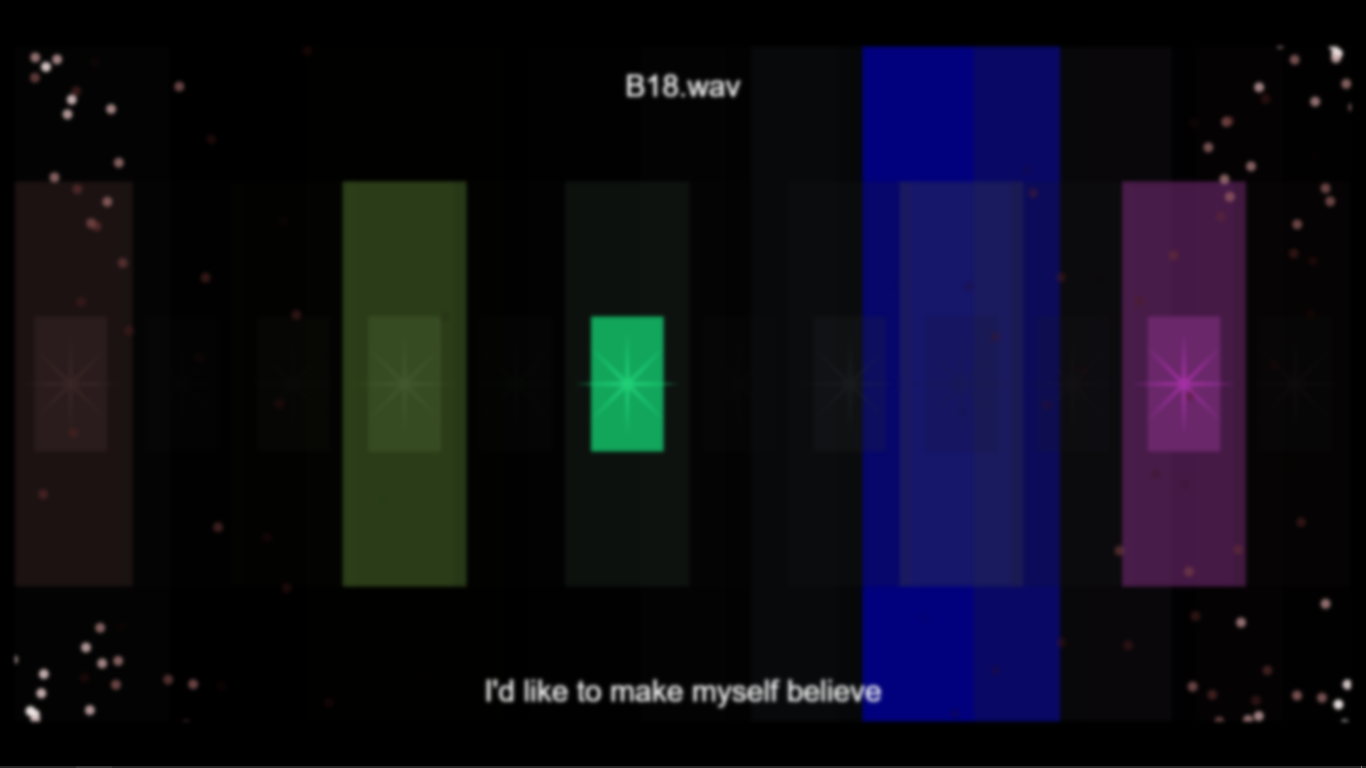
\includegraphics[width=4.75cm,height=3cm]{figures/Prot3.png}
  \caption{A sample screenshot of the visualizer prototype. The visualizations exhibit a high degree of layer independence which has been observed to coincide with decreased upsetness and boredom.}
    \label{fig:prot3_1}
    \end{minipage}
\end{marginfigure}

\begin{marginfigure}[1pc]
\begin{minipage}{\marginparwidth}
     \centering
    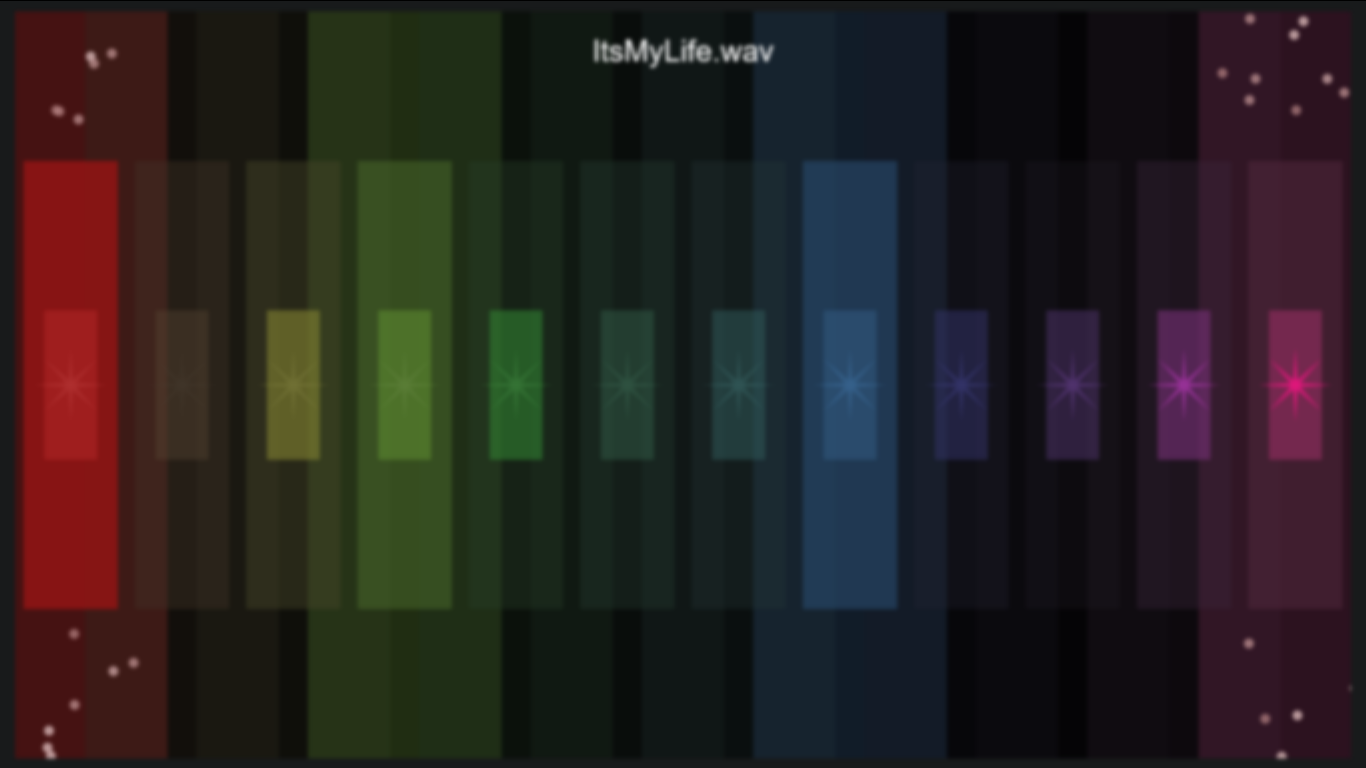
\includegraphics[width=4.75cm,height=3cm]{figures/LowLayerIndependence.png}
  \caption{The visualizations exhibit a high degree of rectangle contiguity which has been observed to coincide with decreased boredom and happiness.}
    \label{fig:prot3_2}
    \end{minipage}
\end{marginfigure}

\begin{marginfigure}[1pc]
\begin{minipage}{\marginparwidth}
     \centering
    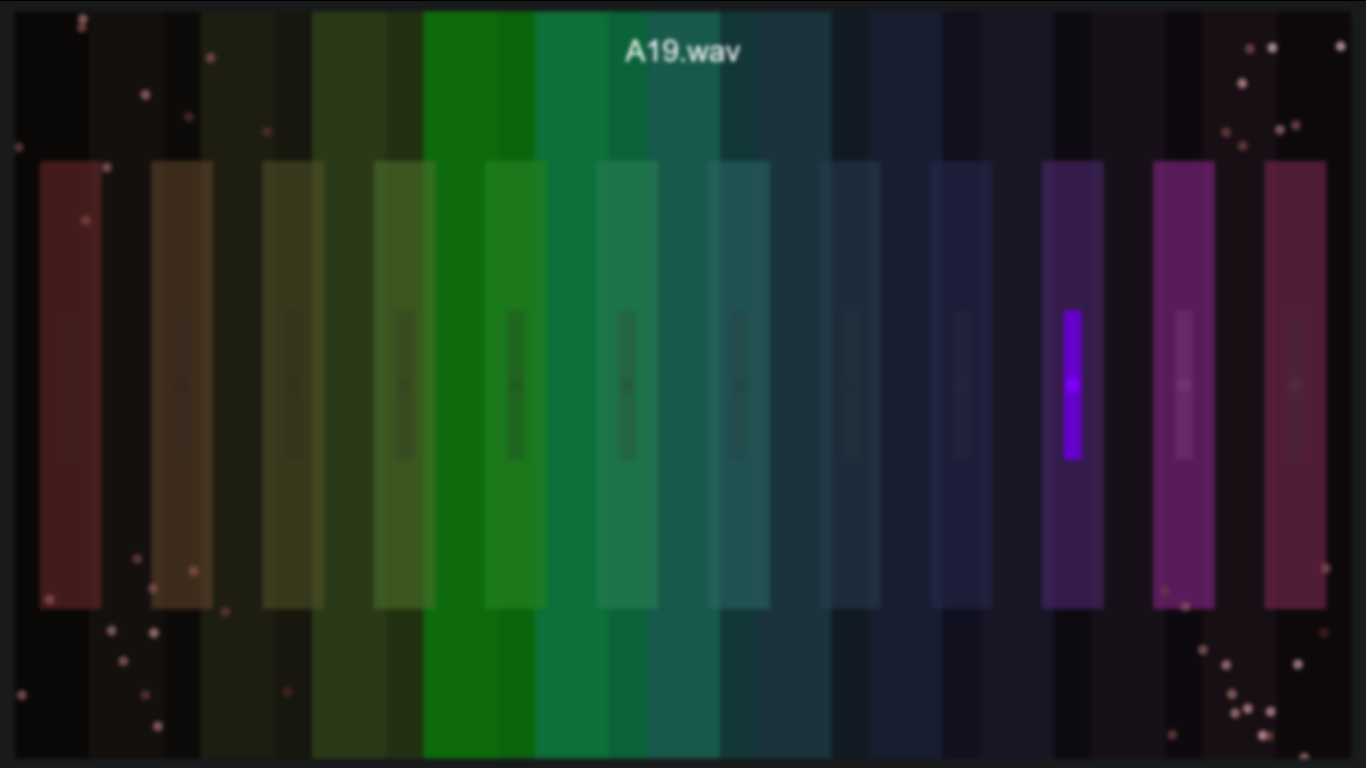
\includegraphics[width=4.75cm,height=3cm]{figures/Predictable.png}
  \caption{The visualizations exhibit a high degree of movement predictability which has been observed to coincide with decreased happiness and increased boredom.}
    \label{fig:prot3_3}
    \end{minipage}
\end{marginfigure}

% %% For the camera ready, use the commands provided by the ACM in the Permission Release Form.

% \CopyrightYear{2020} 
% \acmYear{2020} 
% \setcopyright{rightsretained} 
% \acmConference[CHI'20 Extended Abstracts]{CHI Conference on Human Factors in Computing Systems Extended Abstracts}{April 25--30, 2020}{Honolulu, HI, USA}
% \acmBooktitle{CHI Conference on Human Factors in Computing Systems Extended Abstracts (CHI'20 Extended Abstracts), April 25--30, 2020, Honolulu, HI, USA}
% \isbn{978-1-4503-6819-3/20/04}
% \doi{10.1145/3334480.3383046}
% %% Then override the default copyright message with the \acmcopyright command.
% \copyrightinfo{\acmcopyright}

\CopyrightYear{2020}
\setcopyright{rightsretained}
\conferenceinfo{CHI'20,}{April  25--30, 2020, Honolulu, HI, USA}
\isbn{978-1-4503-6819-3/20/04}
\doi{10.1145/3334480.3383046}
%% Then override the default copyright message with the \acmcopyright command.
\copyrightinfo{\acmcopyright}


\maketitle

% Uncomment to disable hyphenation (not recommended)
% https://twitter.com/anjirokhan/status/546046683331973120
\RaggedRight{} 

% \begin{comment}
% \subsection{Iteration 1}
% \subsubsection{Prototype Visualizer Design}
% \begin{figure}%[ht]
%   \centering
%     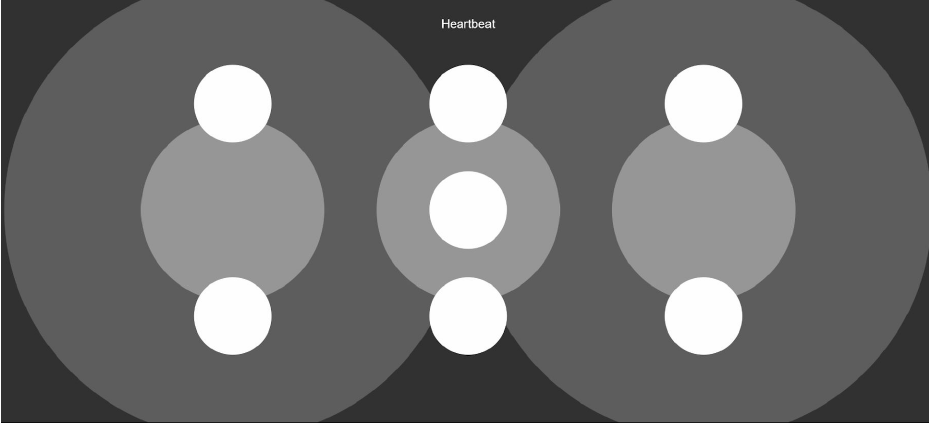
\includegraphics[width=7.5cm,height=4cm]{figures/Prot1.png}
%   \caption{A sample screen of the first prototype}
%   \label{fig:prot1}
% \end{figure}
% \subsubsection{Test Design and Experiment Setup}
% \begin{figure}%[ht]
%   \centering
%     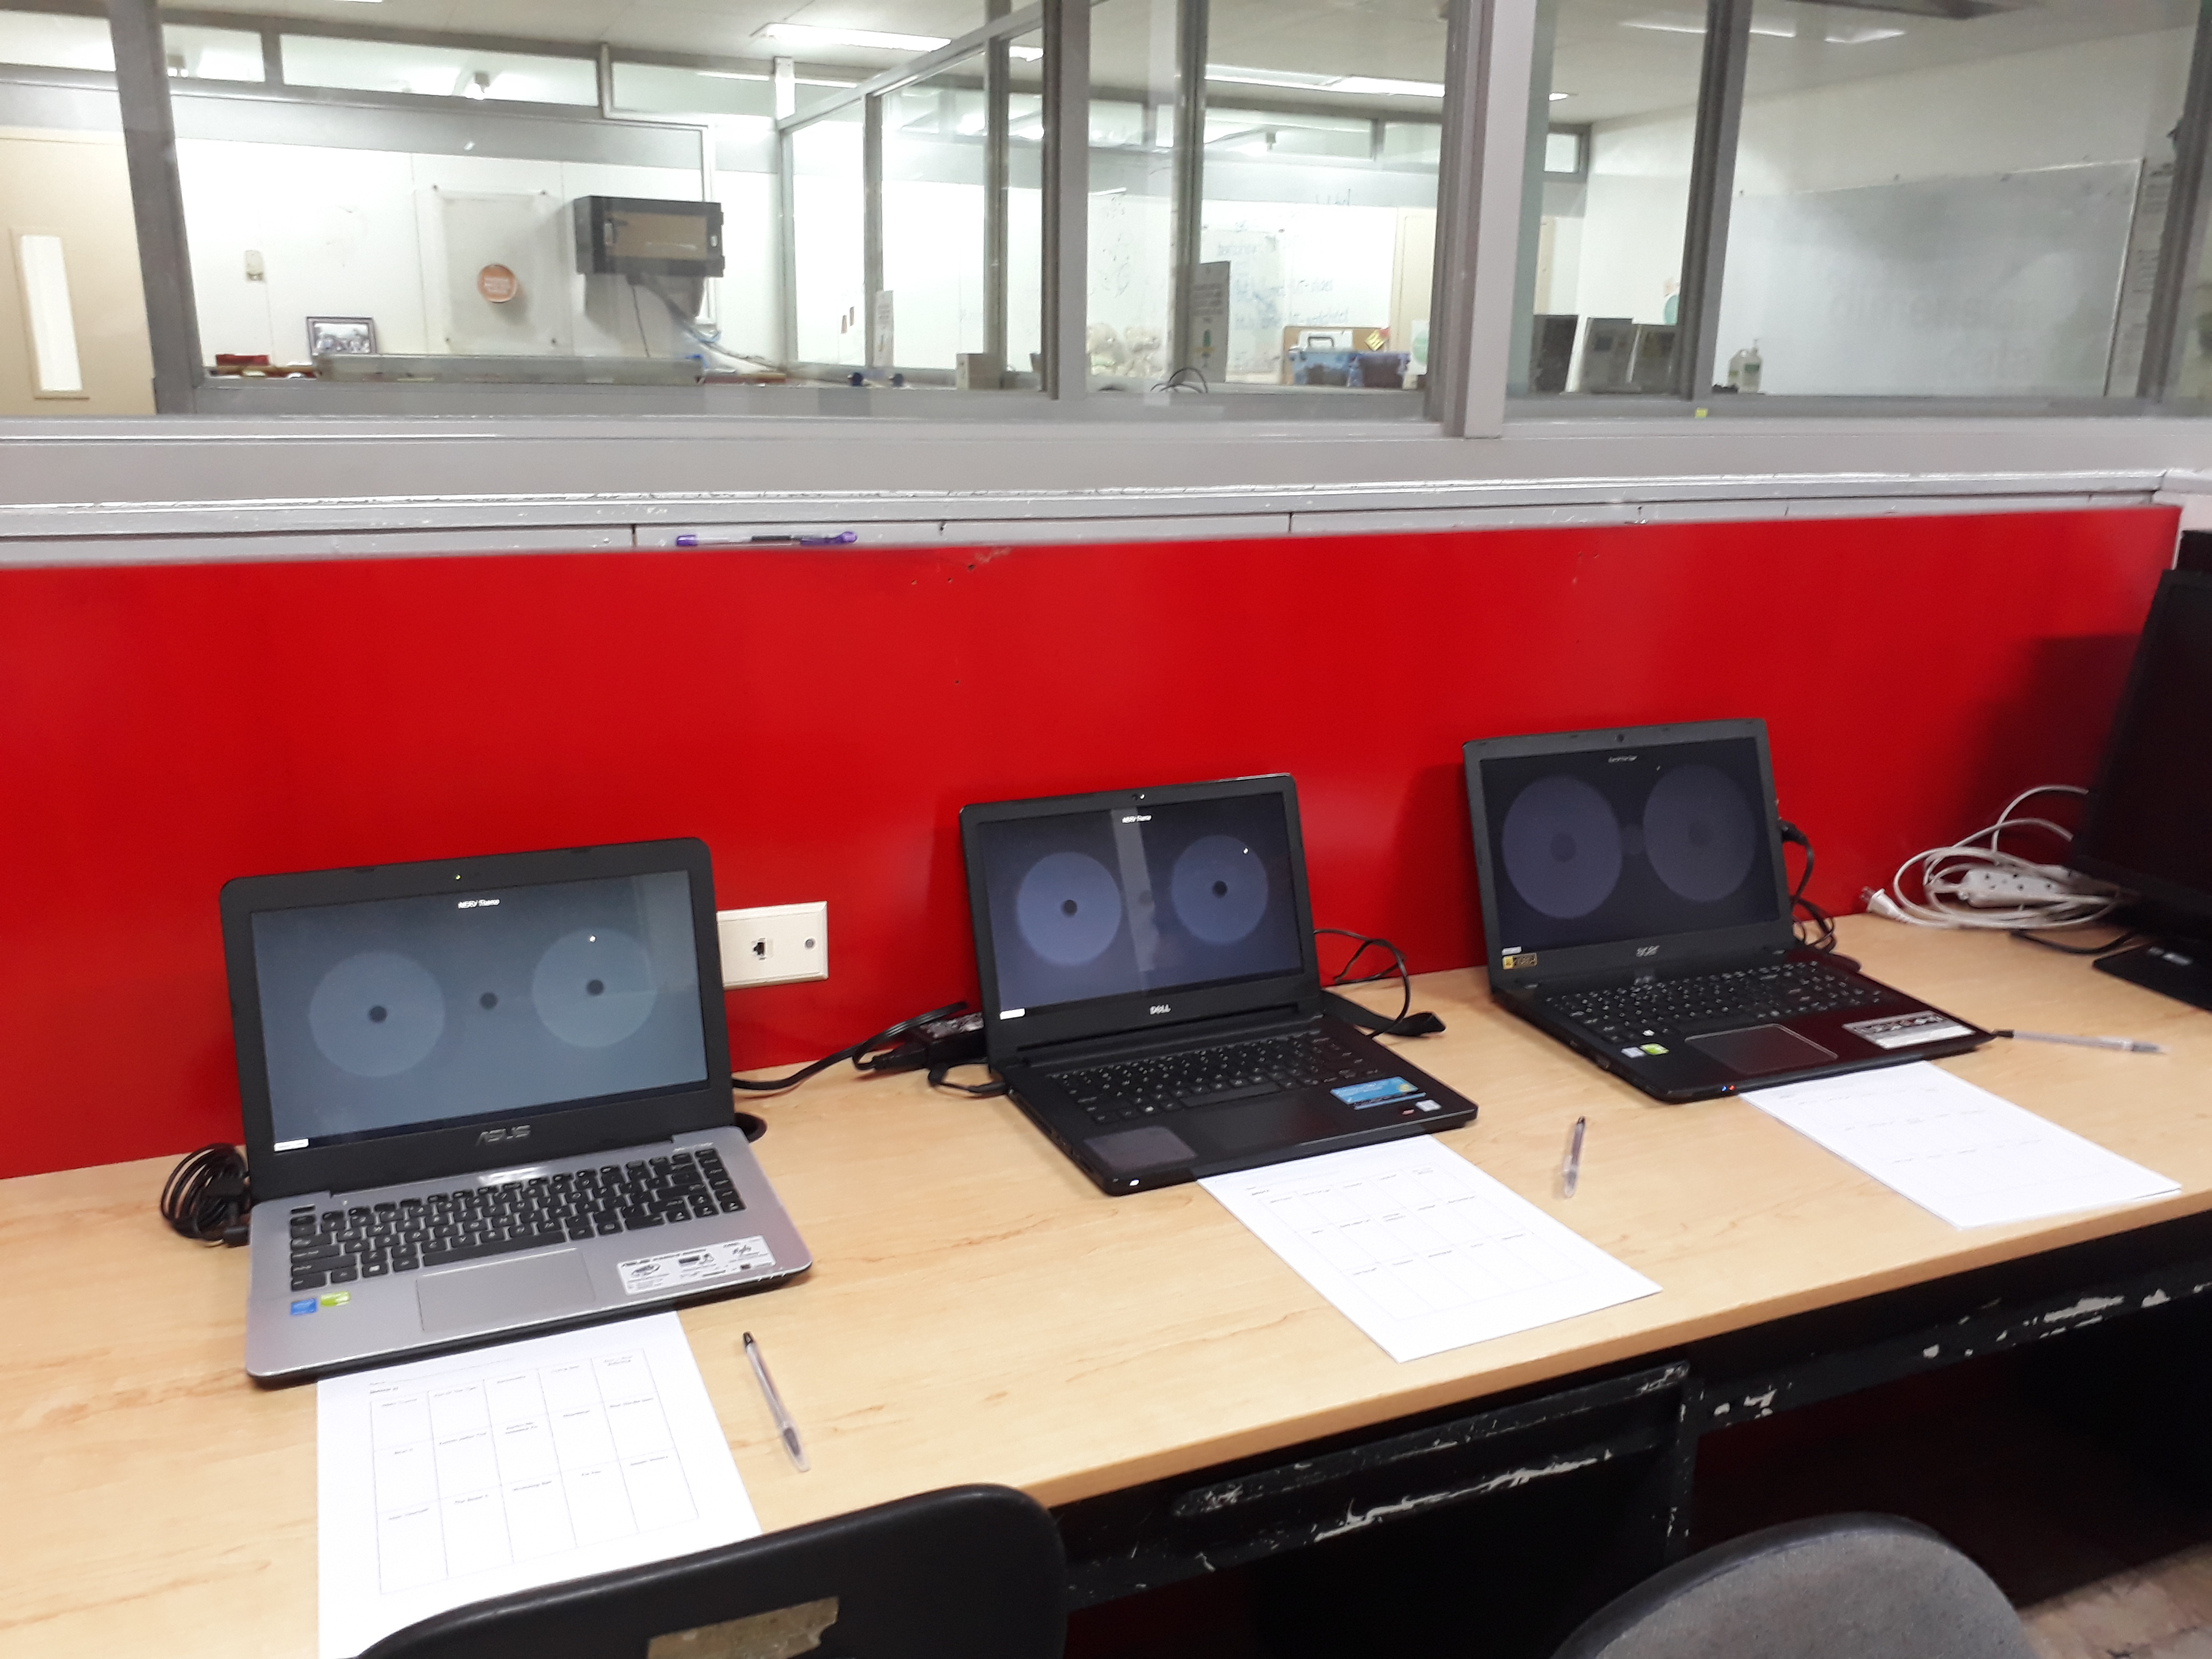
\includegraphics[width=7.5cm,height=4cm]{figures/iter1Setup.jpg}
%   \caption{Experiment setup for iteration 1}
%   \label{fig:iter1Setup}
% \end{figure}

% \subsection{Iteration 2}
% \subsubsection{Prototype Visualizer Design}
% \begin{figure}%[ht]
%   \centering
%     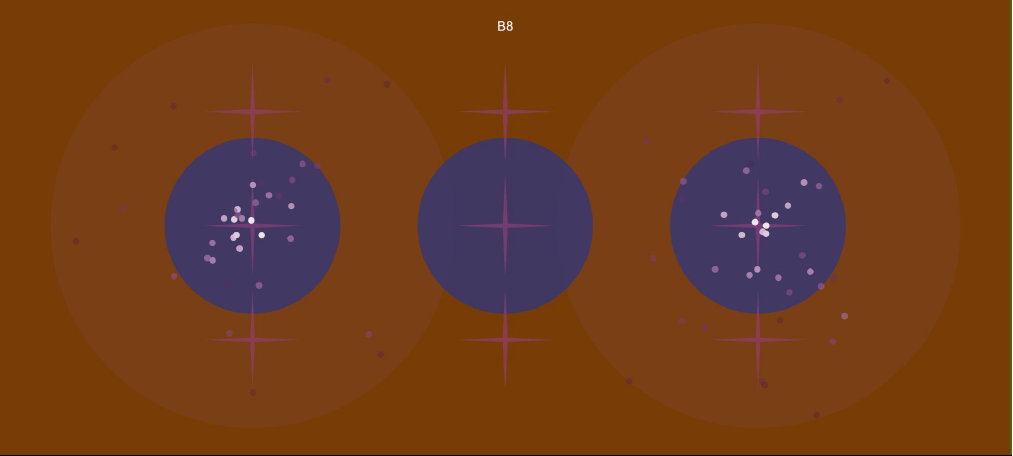
\includegraphics[width=7.5cm,height=4cm]{figures/Prot2.png}
%   \caption{A sample screen of the second prototype}
%   \label{fig:prot2}
% \end{figure}
% \subsubsection{Test Design and Experiment Setup}
% \begin{figure}%[ht]
%   \centering
%     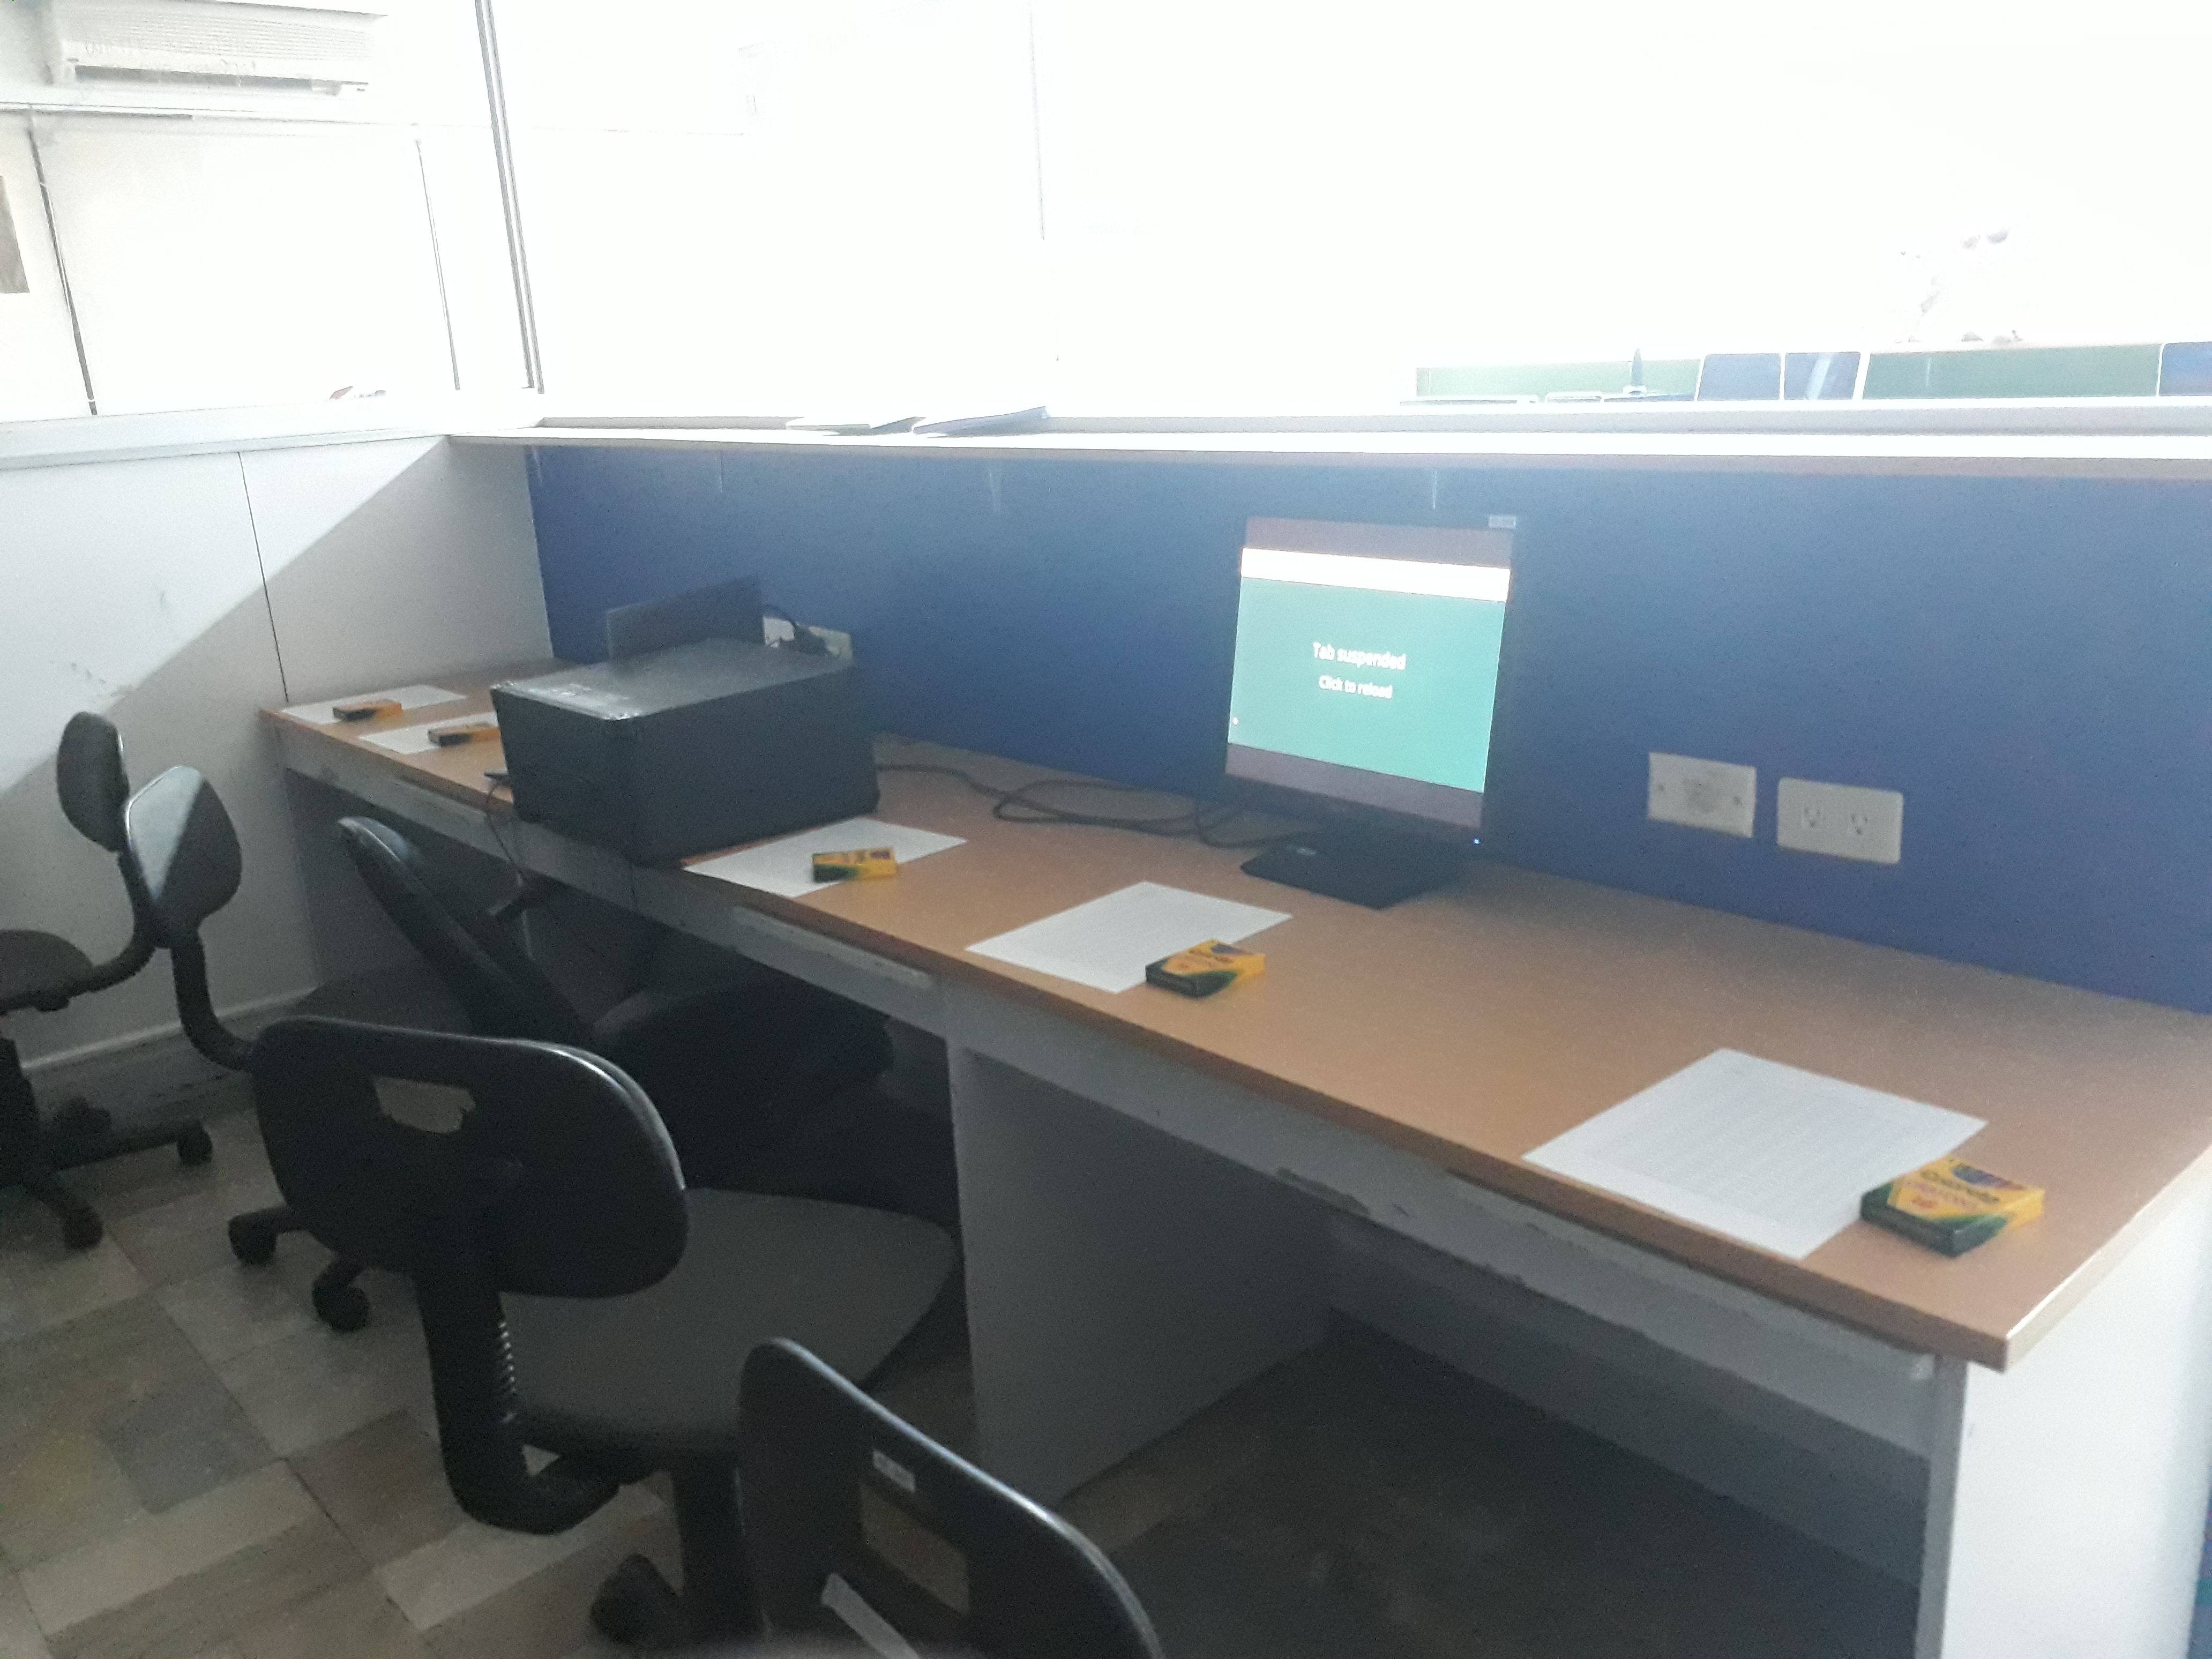
\includegraphics[width=7.5cm,height=4cm]{figures/iter2Setup.jpg}
%   \caption{Experiment setup for iteration 2}
%   \label{fig:iter2Setup}
% \end{figure}

% \subsection{Iteration 3}
% \begin{figure}%[ht]
%   \centering
%     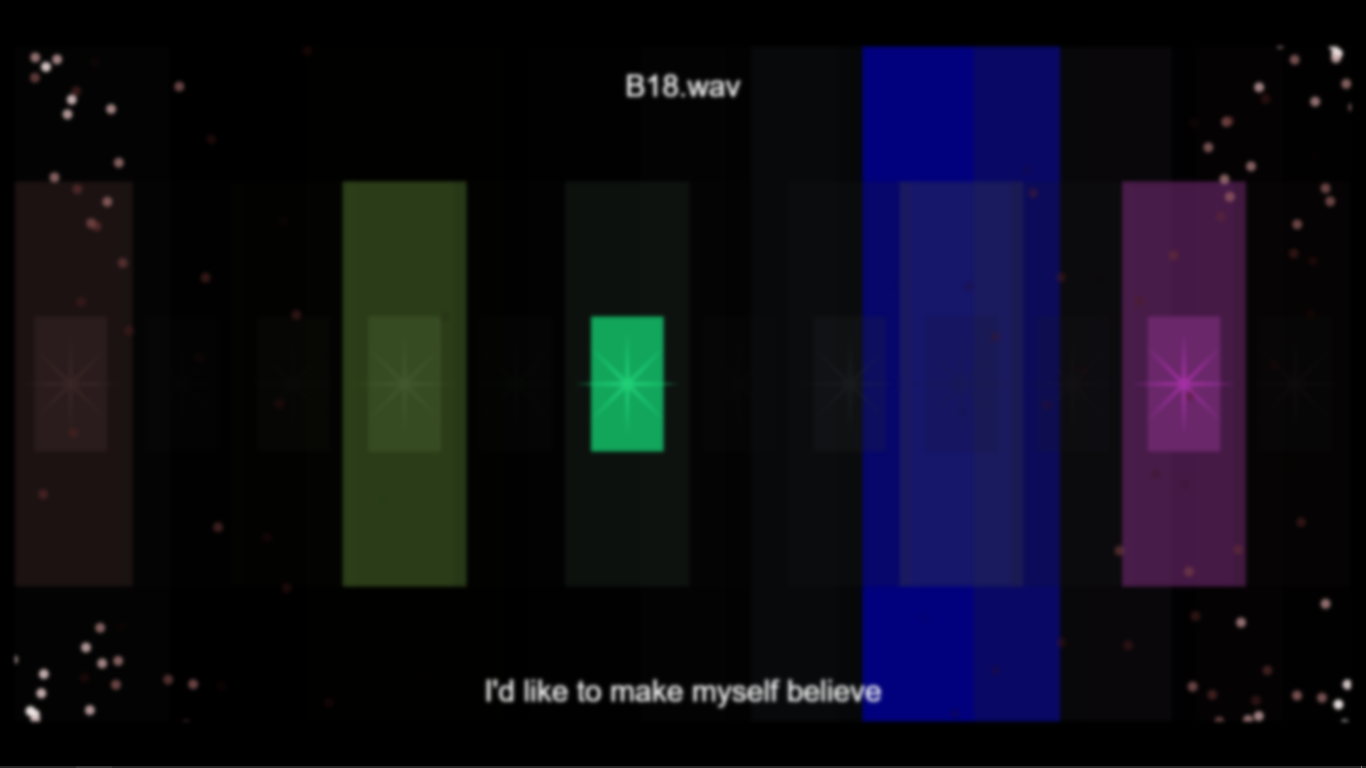
\includegraphics[width=7.5cm,height=4cm]{figures/Prot3.png}
%   \caption{A sample screen of the third prototype}
%   \label{fig:prot3}
% \end{figure}
% \begin{figure}%[ht]
%   \centering
%     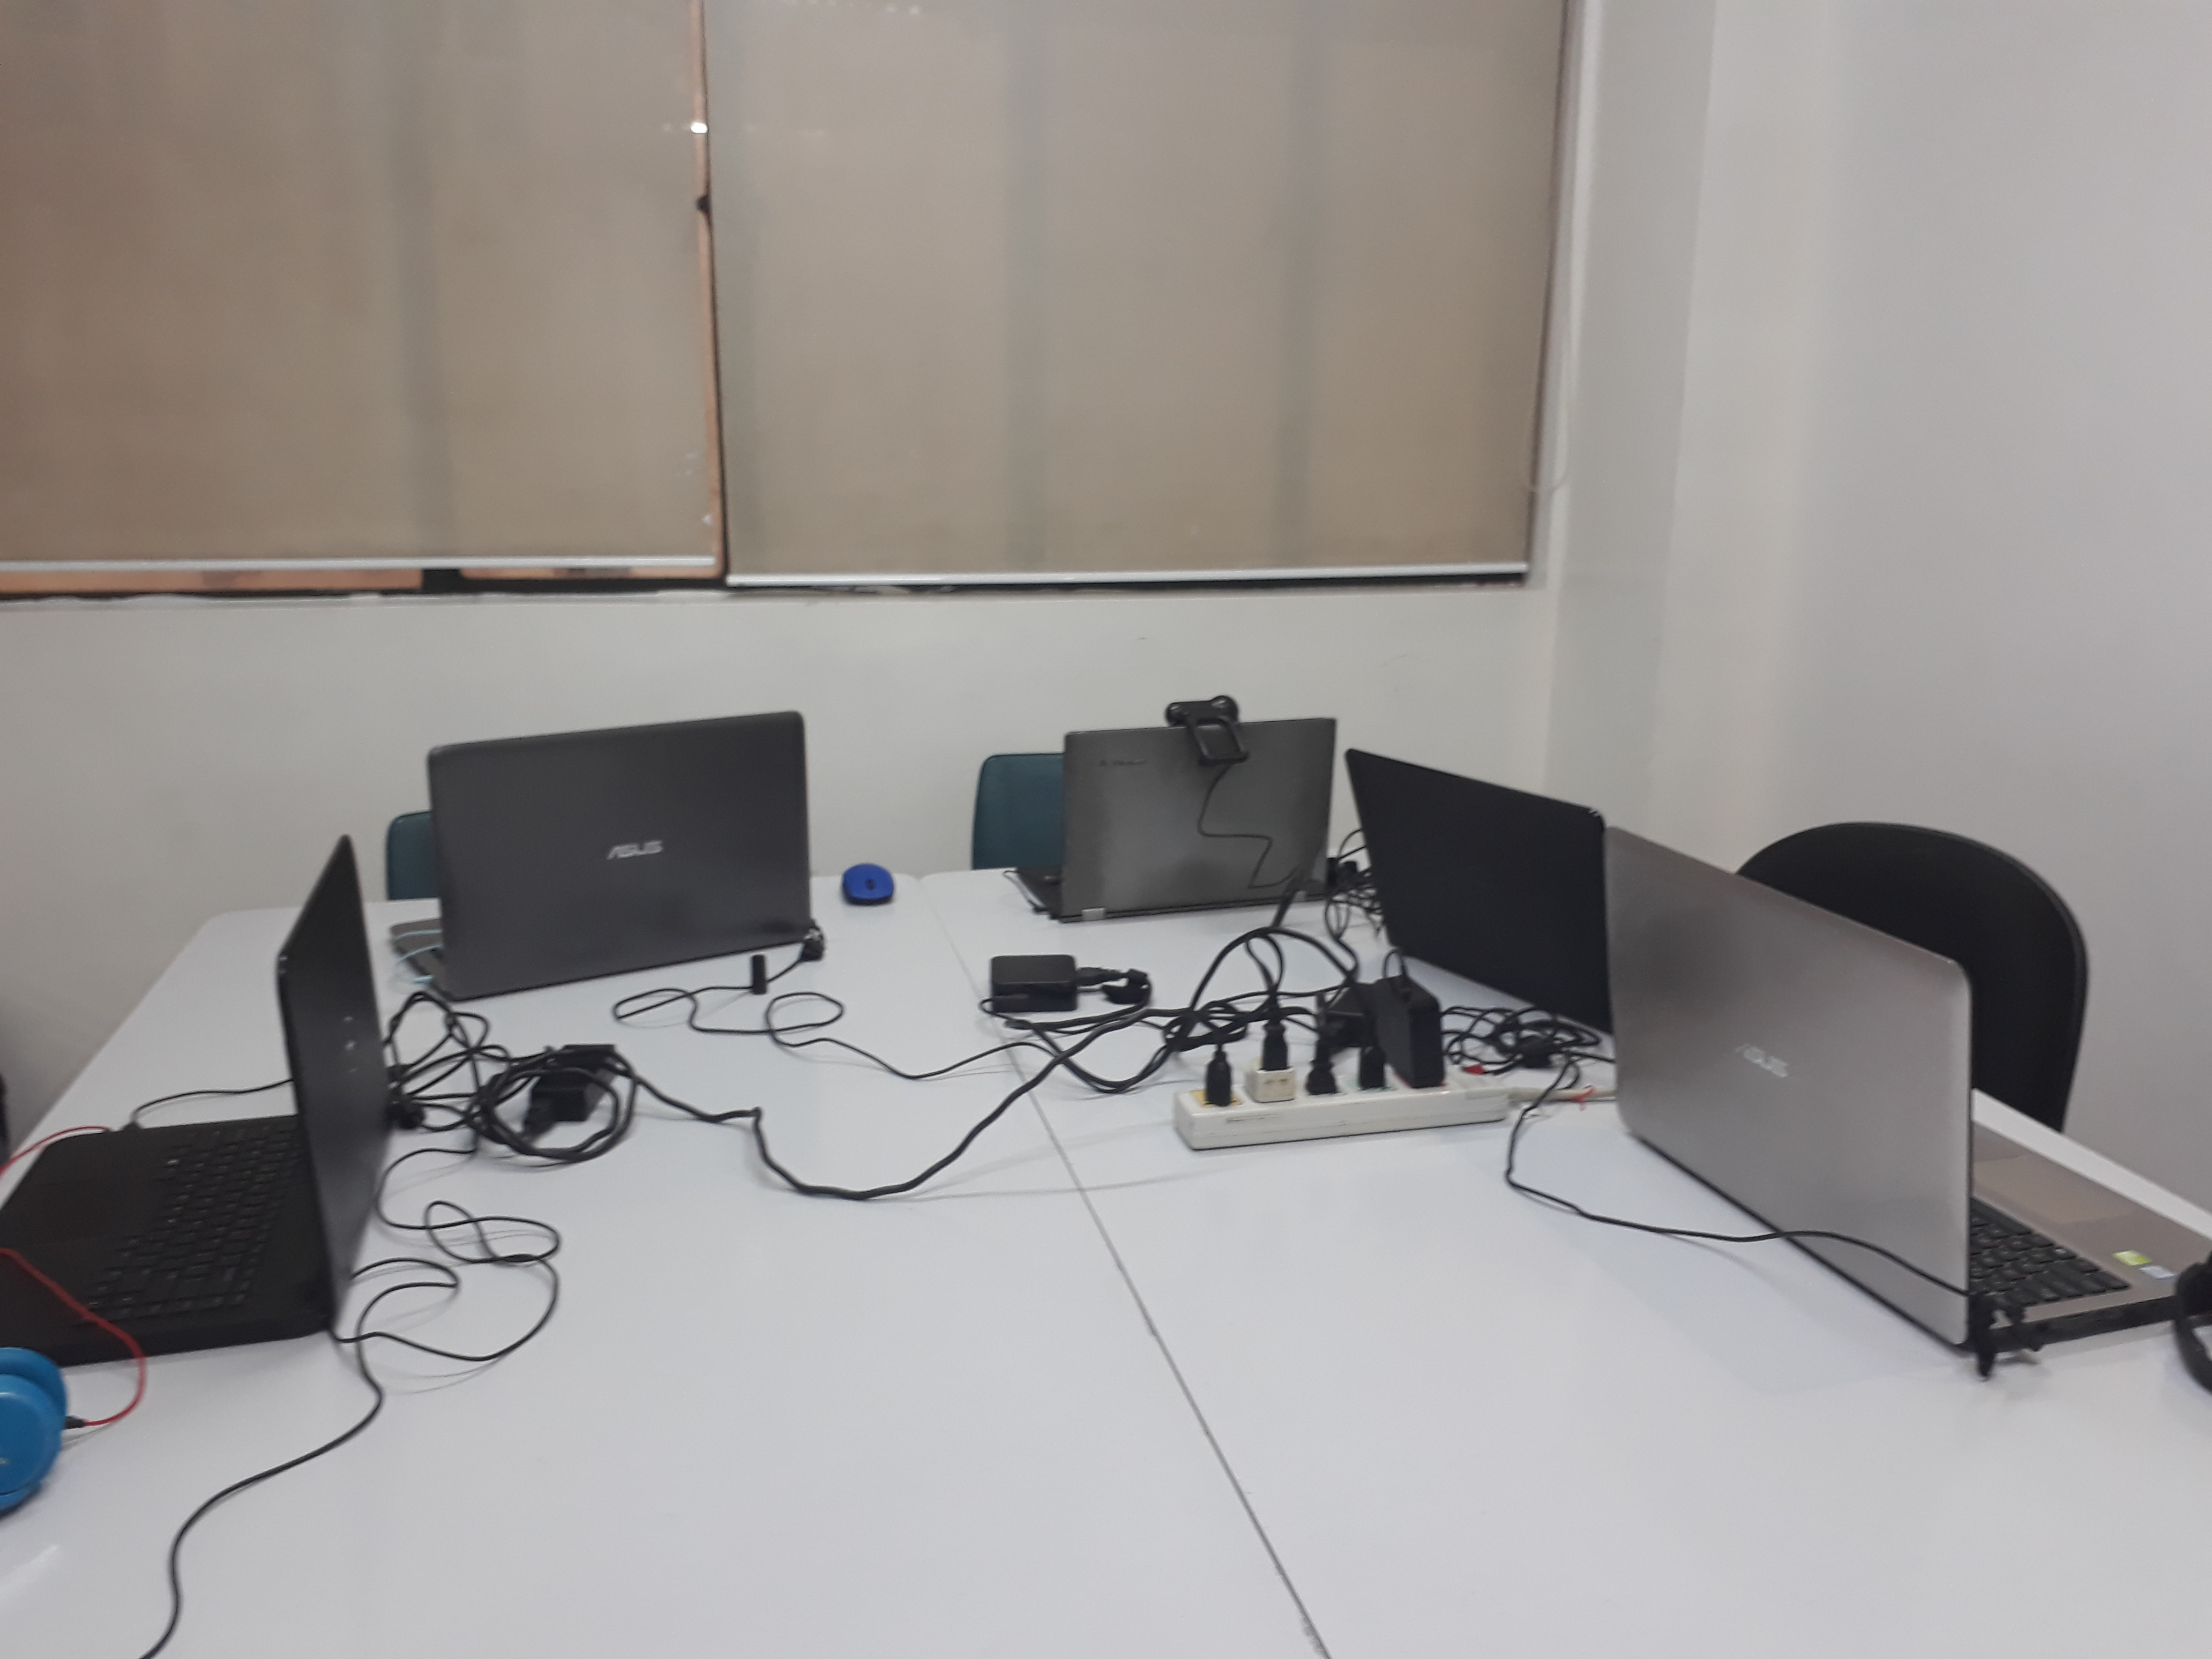
\includegraphics[width=7.5cm,height=4cm]{figures/iter3Setup.jpg}
%   \caption{Experiment setup for iteration 3}
%   \label{fig:iter3Setup}
% \end{figure}
% \end{comment}

% Do not change the page size or page settings.

\begin{abstract}
Visualizers are usually added into music players to augment the listening experiences of hearing users. However, for the case of most members of the Deaf and Hard of Hearing (DHH) community, they have partial deafness which may give them a ``limited'' listening experience as compared to their counterparts. In this paper, we present ViTune, a visualizer tool that enhances the musical experiences of the DHH through the use of an on-screen visualizer generating effects alongside music. We observed how members of the DHH community typically experienced music through an initial user study. We then iterated on developing a visualizer prototype where we did multiple usability tests involving at least 15 participants from the DHH community. We observed how they experienced music with the help of our prototype and noticed that certain music features and elements augmented these experiences. Visualization attributes, their matching qualitative descriptions and equivalent subjective attributes were identified with the help of music experts. Also, affects hypothesized to be induced and dissuaded were identified in improving these listening experiences.
%These graphics were based on related attempts on music visualization and were then designed specifically for the DHH community through an iterative testing and feedback process. A total of 15 participants from the DHH community  As of the latest iteration, we were able to identify visualization characteristics which coincided with the experience of specific affects. For future work, we plan on incorporating the visualizer system with haptic devices, validating the visualizer with an automated testing methodology, comparing the prototype with currently existing music visualizers, and integrating the features of the visualizer into a music player software.
\end{abstract}

\keywords{\plainkeywords}

\begin{CCSXML}
<ccs2012>

<concept>
<concept_id>10003120.10003145.10011770</concept_id>
<concept_desc>Human-centered computing~Visualization design and evaluation methods</concept_desc>
<concept_significance>500</concept_significance>
</concept>

<concept>
<concept_id>10010405.10010469.10010475</concept_id>
<concept_desc>Applied computing~Sound and music computing</concept_desc>
<concept_significance>300</concept_significance>
</concept>

<concept>
<concept_id>10011007.10011074.10011092.10010876</concept_id>
<concept_desc>Software and its engineering~Software prototyping</concept_desc>
<concept_significance>100</concept_significance>
</concept>

</ccs2012>
\end{CCSXML}

\ccsdesc[500]{Human-centered computing~Visualization design and evaluation methods}
\ccsdesc[300]{Applied computing~Sound and music computing}
\ccsdesc[100]{Software and its engineering~Software prototyping}

% Print the classficiation codes
\printccsdesc
% Please use the 2012 Classifiers and see this link to embed them in the text: \url{https://dl.acm.org/ccs/ccs_flat.cfm}

\begin{marginfigure}[0pc]
\begin{minipage}{\marginparwidth}
     \centering
    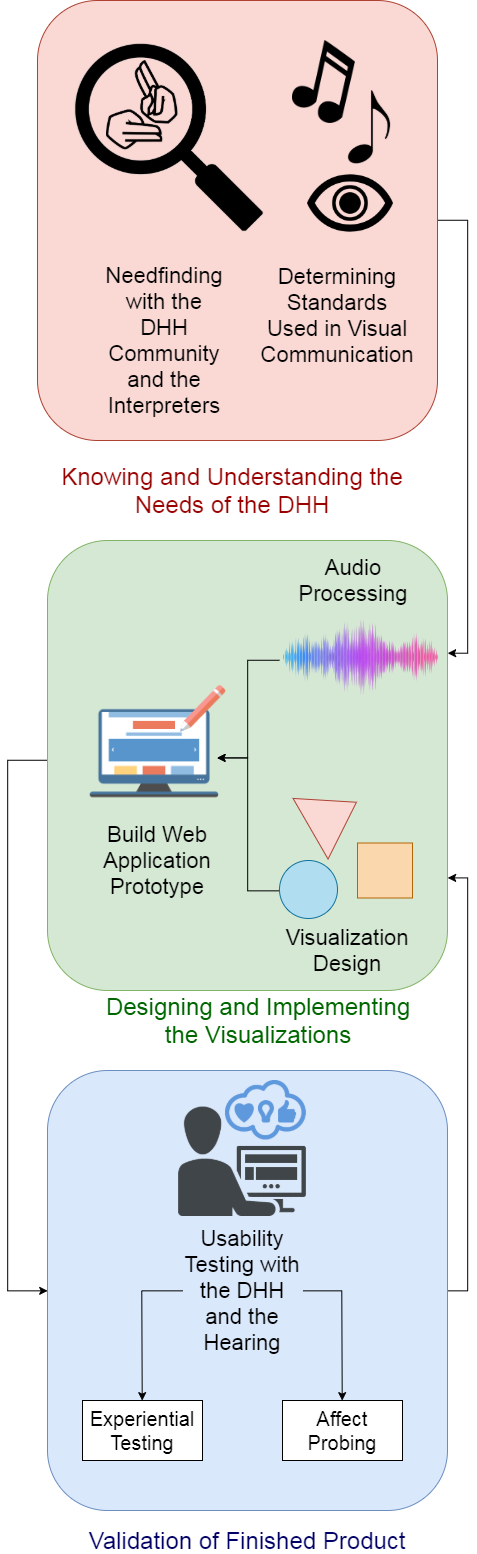
\includegraphics[width=4.5cm,height=12.5cm]{figures/newSystemDesignFlowchart.png}
    \caption{Overview of the Proposed Research Protocol, that is user-centric, iterative, and inclusive. The intended approach as inspired from the work of \protect\cite{deja2019myosl} considers a Human-Centric approach that involves members of the DHH community all throughout the major iterations of the study.}
    \label{fig:methodology}
    \end{minipage}
\end{marginfigure}

\section{Introduction and Related Work}

Members of the DHH community are unable to hear music in its entirety by conventional means. This can lead to different emotional and social difficulties, such as expressing emotions \cite{Nelson:2016, Walker:2013}, making meaningful social connections, and even recognizing the environment and culture they belong to \cite{Gfeller:2012, Ribiero:2017}. The goal of this study is to investigate how members of the DHH community experience music beyond conventional means and determine if these experiences can be augmented with the use of specialized graphics and features.  We intend to answer the research question: \textit{"How might we create an inclusive, effective, and viable visualization system of music for the Deaf and Hard of Hearing?"}. A framework is introduced following the inclusive approach used by \cite{deja2019myosl}, and current work is discussed along with the proposed next steps. There have been two major approaches towards augmenting the musical experience of the DHH community. The first is through the use of \textit{haptic devices} \cite{Balandra:2016}, such as haptic chairs. These allow users to sit on and directly feel musical features through vibrational devices placed on select areas of the said chairs \cite{Nanayakkara:2009:EME}. A modified version of the haptic chair was later developed, wherein the position of the produced vibrations is dependent on the pitch of the music \cite{Jack:2015}. The majority of research already explores haptic technology in their work. This paper exploits the opportunity given the limited work with \textit{visual displays}.
There are usually two presentation types used in music visualization. One is the \textit{piano roll}, which shows a timeline of notes and musical events for a short period of time. It also introduces future events which show up on one end of the screen while eventually scrolling to the other end. The other type is the \textit{movie roll}, which takes up the entire screen space. It only shows the events that are currently taking place during a particular instance, allowing for more creative visuals. \cite{Nanayakkara:2007} notes that it is a more appropriate option for augmenting experiences. Aside from an experiential visualizer attempt, other works on visualizations for music and for the DHH have been done \cite{Fonteles:2013,Jain:2015,Petry:2016}. One work proposed a particle emitter visualization to help with music understanding \cite{Fonteles:2013}. Visualizations were also shown on a head-mounted display to help the DHH with sound awareness as seen in the work of \cite{Jain:2015}. Much of the work on this area can still be improved by emphasizing the role and feedback of the DHH community continuously throughout the development process, as we draw inspiration from the informal notion of \textit{images that we can hear}.

\section{Methodology}
The methodology used in this study can be seen as described in Figure \ref{fig:methodology}. We follow three major phases. The approach used for this methodology is inspired by the framework designed in the study by \cite{deja2019myosl}. We follow an iterative approach in developing the prototype. Members of the DHH community participated and gave their feedback on the different phases of the study (as seen in the green and blue rectangles in Figure \ref{fig:methodology}).

\paragraph{System Design}\mbox{} \\
What we refer to as the visualizer prototype is actually composed of two major modules: the \textbf{analyzer} module, and an actual \textbf{visualizer} module. The analyzer module is responsible for performing audio preprocessing on the music file, while the visualizer module is responsible for the actual visualization of the music file driven by interpreting the analysis made by the analyzer module. See Figure \ref{fig:architecture} for a diagram of the prototype architecture.



The analyzer module accepts the music file to be visualized and, optionally, a file containing manually transcribed lyrics corresponding to the given music file. 

\begin{marginfigure}[-8pc]
\begin{minipage}{\marginparwidth}
     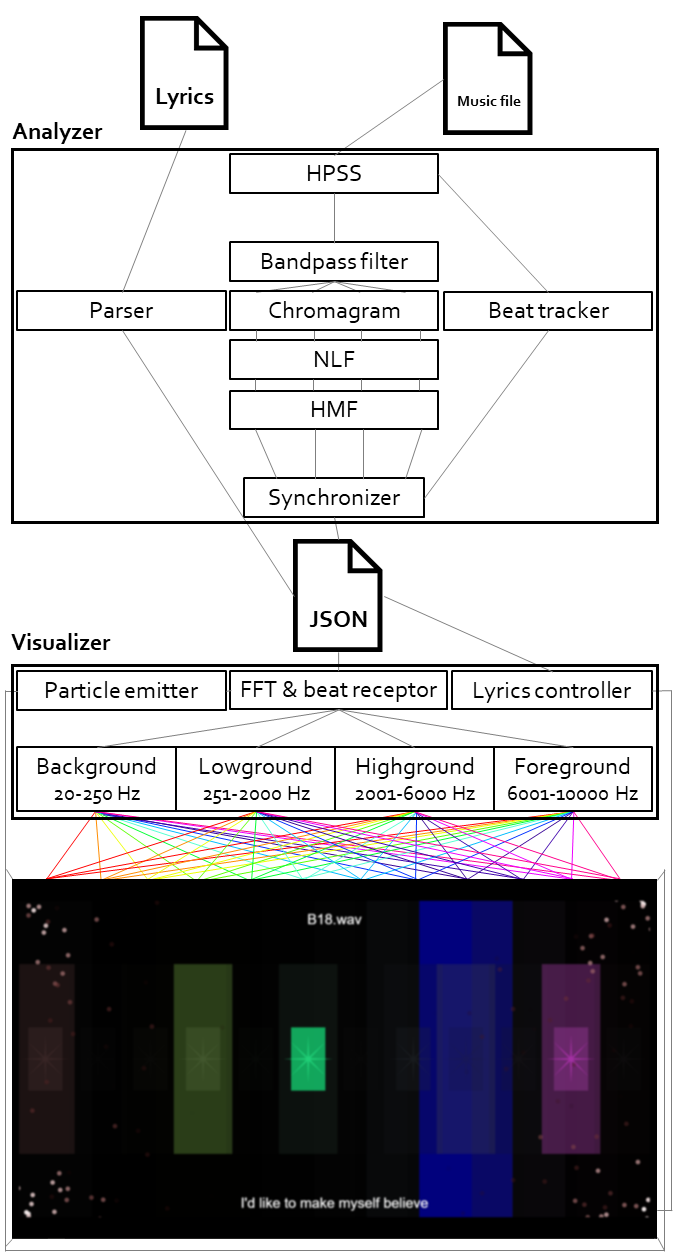
\includegraphics[width=4.75cm,height=8cm]{figures/ArchitectureLBW.png}
    \caption{A simplified diagram of the visualizer prototype architecture.}
    \label{fig:architecture}
    \end{minipage}
\end{marginfigure}

\begin{marginfigure}[0.5pc]
\begin{minipage}{\marginparwidth}
     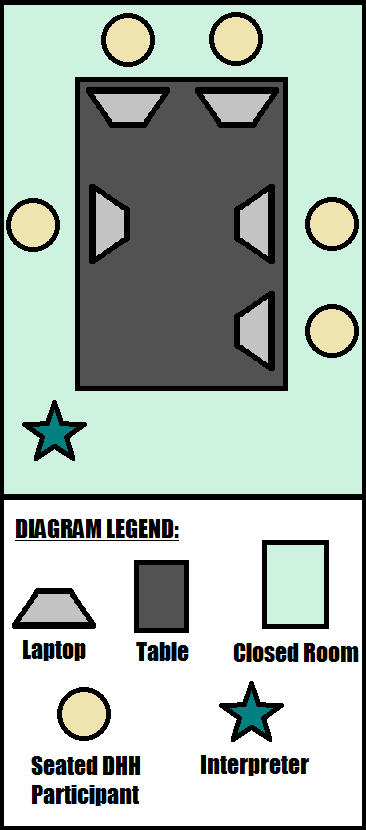
\includegraphics[width=4.5cm,height=8.5cm]{figures/iter3SetupVector.png}
    \caption{The experiment setup for the third iteration.}
    \label{fig:iter3SetupVector}
    \end{minipage}
\end{marginfigure}

All audio processing in this module was done using Librosa, a Python package for music and audio analysis described in \cite{McFee:2015}. The analyzer first performs harmonic-percussive source separation (HPSS). Bandpass filters then divide the harmonic components into four frequency classifications based on the audio spectrum as discussed by \cite{Leigh:2018}. These classifications are: the \textbf{background} (20-250 Hz), representing the sub-bass and bass bands; the \textbf{lowground} (251-2000 Hz), representing the low-midrange and midrange bands; the \textbf{highground} (2001-6000 Hz), representing the upper-midrange and presence bands; and the \textbf{foreground} (6001-10000 Hz), representing a part of the brilliance band. Each of the harmonic components corresponding to each of these classifications are created a chromagram. The chromagrams are subjected to non-local filtering (NLF) and horizontal medium filtering (HMF) to reduce noise. Finally, the chromagram frames are synchronized with the beat frames based on the tempo as estimated by the beat tracker on the percussive component of the music file. The chromagrams, along with the lyrics, if provided, are now packaged into a JSON file for visualization. The visualizer module takes the JSON file containing the results of the analysis as an input. Unlike in the preprocessing phase, the audio processing done in this module is done in real time (i.e., \textit{while} the music is playing). As the music file is played by this module, a Fast Fourier Transform (FFT) is used to once again separate the current audio frame into the four frequency classifications we mentioned earlier. The mean signal strength per frame of each classification (changed per audio frame in real time) is used to determine the size of the classification's visualization layer components, while the chromagrams from the analyzer are used to determine the saturation, brightness, and opacity of the visualization layer components (changed per music beat). For all but the foreground layer, each classification's visualization layer is composed of rectangular columns. Stars compose the visualization layer of the foreground. Particle emitters are activated when the signal strengths in the foreground layer (expected to contain the percussive parts of the music) experience a spike within a short period of time.



\paragraph{Usability Evaluation}
\subsection{Initial User Research}
Prior to any prototype development and testing, we conducted initial user research through needfinding and some structured interviews. We did this to acquire preliminary insights from members of the DHH community with the help of sign language interpreters. Some insights were also drawn from surveys and questionnaires filled up by other members of the DHH community.  Questions in the survey inquired about their preferences on which types of visuals were appealing.


\subsection{Music Selection and Classification}
A playlist was crafted based on the preferences of the DHH participants. We gathered 106 MP3 files encompassing a variety of genres, each of which were subjectively reviewed and classified based on their characteristics with the help of music experts. In determining the music to be eliminated from the playlist, we played each musical piece through the first visualizer prototype. The general animation patterns and shapes present were noted, and the musical pieces which were deemed to be unremarkably visualized were ruled out. The final playlist was narrowed down to a total of 25 musical pieces. These samples were diverse in terms of tempo, rhythm, loudness, genre, and the presence of vocals. For the third and final iteration prototype, the playlist was further narrowed down to 15 musical pieces using the same process while also taking into account the feedback of the DHH community during the previous iterations with respect to how the musical pieces were visualized.




\begin{marginfigure}[0pc]
\begin{minipage}{\marginparwidth}
     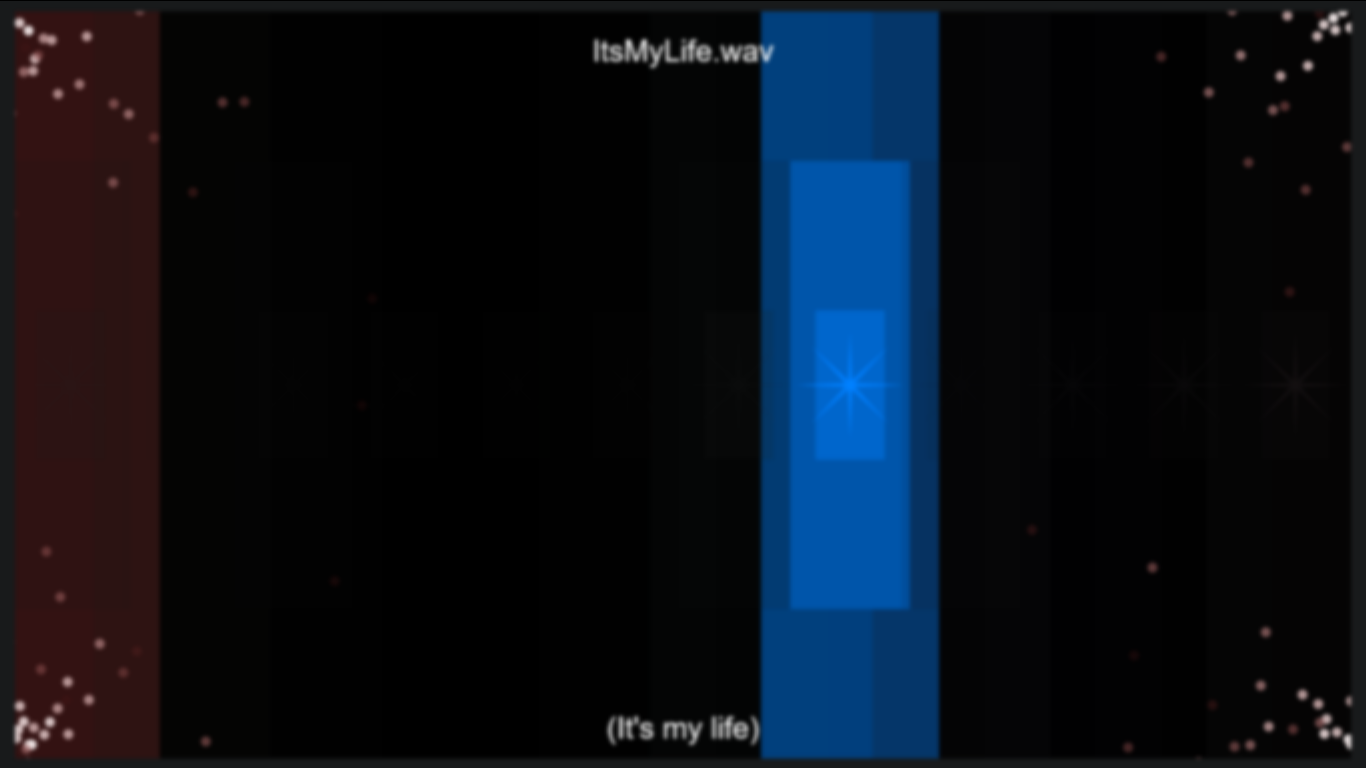
\includegraphics[width=4.5cm,height=3cm]{figures/LowParticleActivity.png}
    \caption{Low particle activity is exhibited by the visualizer as shown in this screenshot.}
    \label{fig:lowparticle}
    \end{minipage}
\end{marginfigure}

\begin{marginfigure}[0pc]
\begin{minipage}{\marginparwidth}
     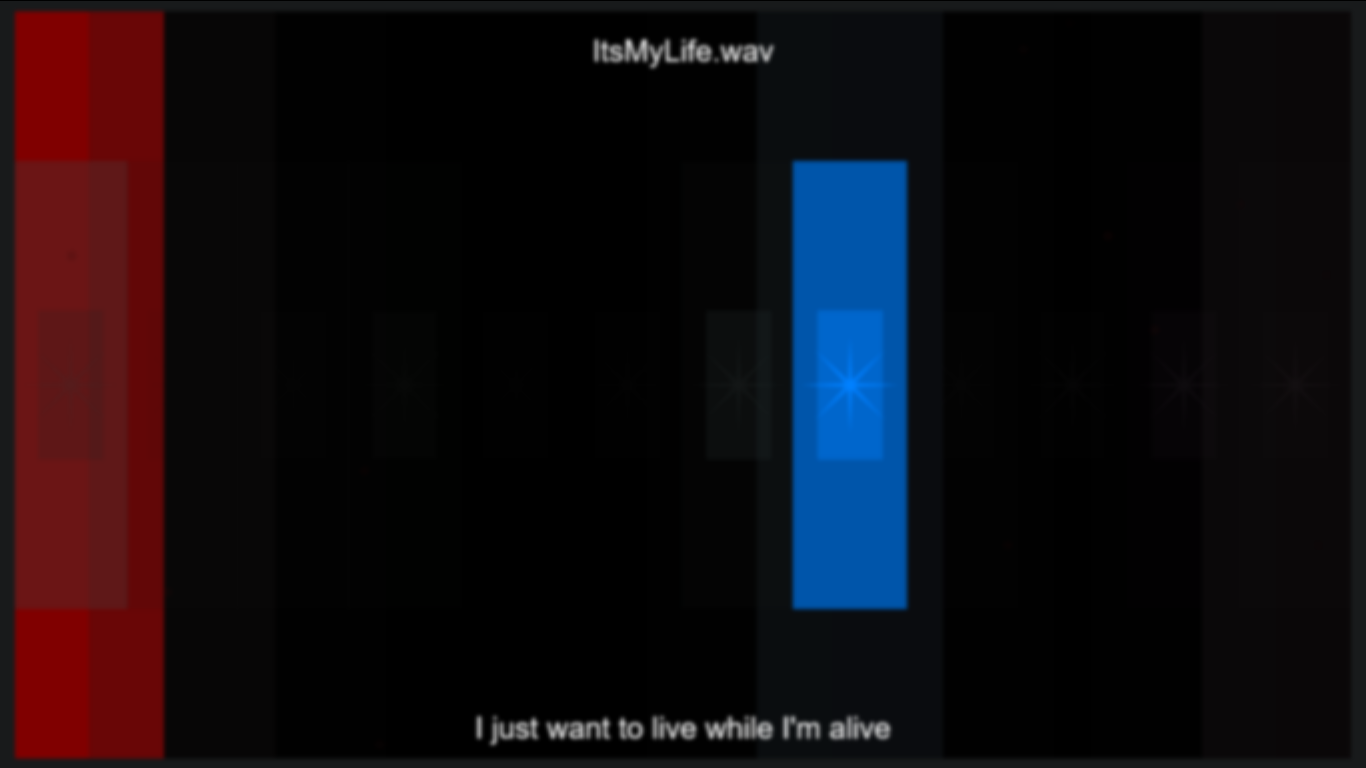
\includegraphics[width=4.5cm,height=3cm]{figures/LowStarVsisibility.png}
    \caption{Low star prominence is exhibited by the visualizer as shown in this screenshot.}
    \label{fig:lowstar}
    \end{minipage}
\end{marginfigure}

\begin{marginfigure}[0pc]
\begin{minipage}{\marginparwidth}
     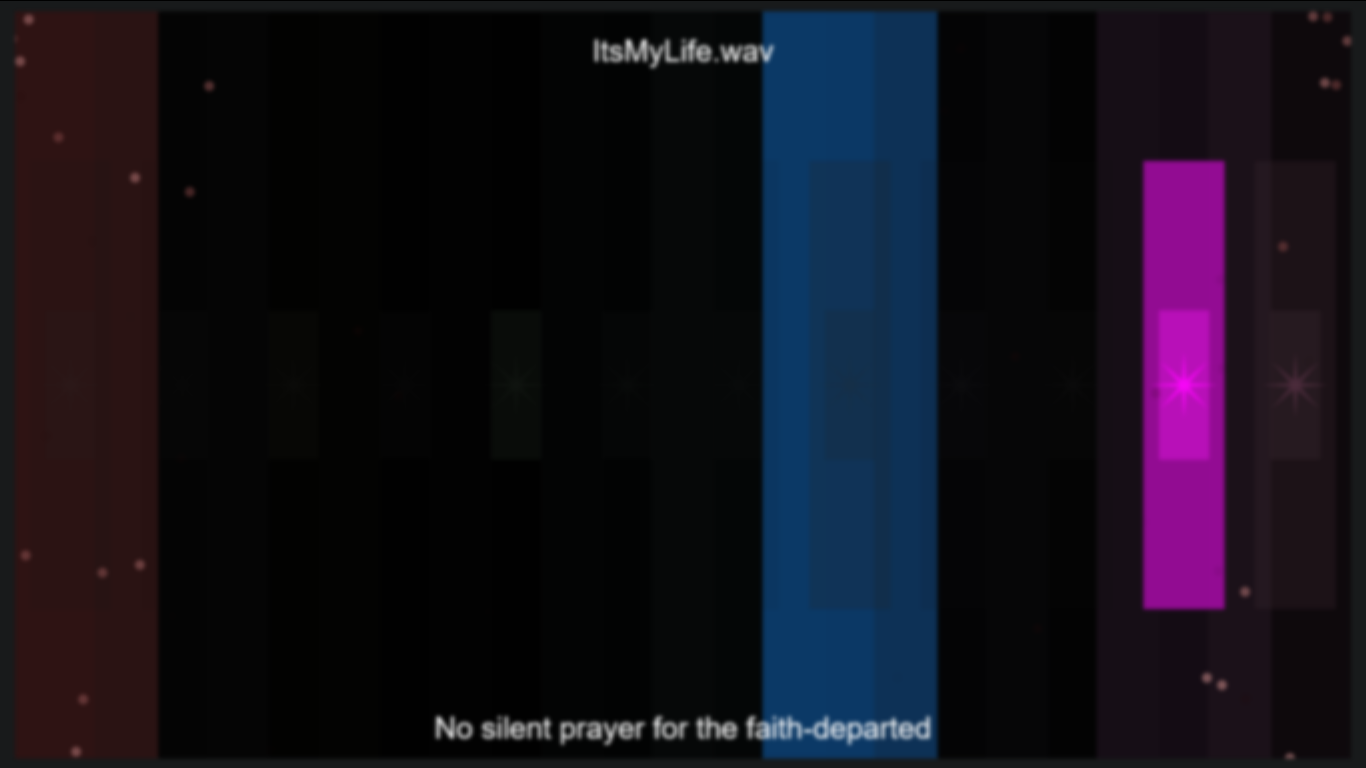
\includegraphics[width=4.5cm,height=3cm]{figures/HighLayerIndependence.png}
    \caption{High layer independence is exhibited by the visualizer as shown in this screenshot.}
    \label{fig:highindependence}
    \end{minipage}
\end{marginfigure}

% \begin{marginfigure}[-1pc]
% \begin{minipage}{\marginparwidth}
%      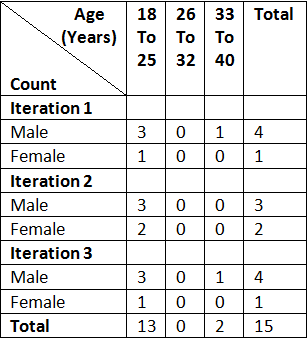
\includegraphics[width=4.5cm,height=5cm]{figures/participant_demographics_vertical.png}
%     \caption{The breakdown of the participants throughout the three (3) iterations.}
%     \label{fig:participants}
%     \end{minipage}
% \end{marginfigure}



\subsection{Iterative Prototype}
A visualizer prototype was developed using the results and insights gathered from at least two previous versions. For inclusivity, web technologies are used for the development of the prototype. Based on feedback, adjustments were made to the graphic visualizations based on the music features considered. These adjustments were incorporated into a visualization format and architecture based on previous works. The background was set to black and the screen was divided vertically into twelve rectangular columns, mapped to the color spectrum (red to violet) from left to right. Each column contains smaller visual elements: two smaller rectangles and a star. These twelve columns represent the frequencies, falling in one of the twelve pitch classes (C to B) present in the music at the current time. The choice to map the note C with the color red is arbitrary since \cite{Evans:2005} states that there is no perceptual hierarchy of hue. The idea of the partitioning of visual elements based on audio frequency is based on \cite{Nanayakkara:2009:EME} and \cite{Nanayakkara:2007}. Particle emitters were positioned at each of the four corners of the screen. This draws inspiration from \cite{Fonteles:2013}. Based on the feedback of the users, lyrics, if there were any, were preferred to appear at the bottom of the screen, synchronized with the vocals (Figure \ref{fig:prot3_1} shows an image sample of the visualization). The initial design of these visualizer components are based on the architecture of \cite{Nanayakkara:2007}.

\subsubsection{Experiment Design and Usability Tests}
During the usability tests, each participant was provided a laptop containing the visualizer prototype, a webcam for facial recording, and earphones or headphones. The layout of the setup can be seen in Figure \ref{fig:iter3SetupVector}. The test design consisted of two phases: (1) prototype testing, and (2) clip review. In the first phase, the participants watched the visualizations generated by the visualizer for each of the 15 musical pieces. While watching, both the visualizations shown on screen and the faces of the participants were recorded simultaneously. A separate tool, made for marking the current time with a button, was created for the tester to click on and was active throughout the entire testing phase. The participants were instructed to click on this button every time they wanted to mark the times wherein the visualizations made them feel ``something''. At the end of each test, participants were asked to reflect on their viewing experiences. This was done by making them watch their own respective recordings. This allowed them to record and label the specific emotion they felt during a specific button click which they have initially marked. By reflecting on their reactions to these visualizations, they were able to accurately label what the visuals made them feel. This allowed them to further describe and elaborate on why they felt that way. The testers were given eight labels of affect to choose from based on the circumplex model of affect by \cite{Russel:1980}. These affects are: excited, happy, contented, relaxed, bored, sad, upset, and tensed.



% \section{Architecture}
% What we refer to as the visualizer prototype is actually composed of two (2) major modules: the \textbf{analyzer} module, and an actual \textbf{visualizer} module. The analyzer module is responsible for performing audio preprocessing on the music file, while the visualizer module is responsible for the actual visualization of the music file driven by interpreting the analysis made by the analyzer module. See Figure \ref{fig:architecture} for a diagram of the prototype architecture.







% The analyzer module accepts the music file to be visualized and, optionally, a file containing manually transcribed lyrics corresponding to the given music file. All audio processing in this module was done using Librosa, a Python package for music and audio analysis described in \cite{McFee:2015}. The analyzer first performs harmonic-percussive source separation (HPSS). Bandpass filters then divide the harmonic components into four (4) frequency classifications based on the audio spectrum as discussed by \cite{Leigh:2018}. These classifications are: the \textbf{background} (20-250 Hz), representing the sub-bass and bass bands; the \textbf{lowground} (251-2000 Hz), representing the low-midrange and midrange bands; the \textbf{highground} (2001-6000 Hz), representing the upper-midrange and presence bands; and the \textbf{foreground} (6001-10000 Hz), representing a part of the brilliance band. Each of the harmonic components corresponding to each of these classifications are created a chromagram. The chromagrams are subjected to non-local filtering (NLF) and horizontal medium filtering (HMF) to reduce noise. Finally, the chromagram frames are synchronized with the beat frames based on the tempo as estimated by the beat tracker on the percussive component of the music file. The chromagrams, along with the lyrics, if provided, are now packaged into a JSON file for visualization. The visualizer module takes the JSON file containing the results of the analysis as an input. Unlike in the preprocessing phase, the audio processing done in this module is done in real time (i.e., \textit{while} the music is playing). As the music file is played by this module, a Fast Fourier Transform (FFT) is used to once again separate the current audio frame into the four frequency classifications we mentioned earlier. The mean signal strength per frame of each classification (changed per audio frame in real time) is used to determine the size of the classification's visualization layer components, while the chromagrams from the analyzer are used to determine the saturation, brightness, and opacity of the visualization layer components (changed per music beat). For all but the foreground layer, each classification's visualization layer is composed of rectangular columns. Stars compose the visualization layer of the foreground. Particle emitters are activated when the signal strengths in the foreground layer (expected to contain the percussive parts of the music) experience a spike within a short period of time.

\section{Results}
\subsection{Participant Demographics}



% \begin{table}[H]
% \label{tab:demographic}
% \begin{tabular}{|c|c|c|c|c|}
% \hline
% \multirow{2}{*}{\textbf{}} & \multicolumn{4}{c|}{\textbf{Age (Years)}} \\ \cline{2-5} 
%                           & 18-25  & 26-32  & 33-40  & \textbf{Total} \\ \hline
% \multicolumn{5}{|c|}{\textbf{1st Iteration Count}}                           \\ \hline
% Male                       & 3      & 0      & 1      & 4              \\ \hline
% Female                     & 1      & 0      & 0      & 1              \\ \hline
% \multicolumn{5}{|c|}{\textbf{2nd Iteration Count}}                            \\ \hline
% Male                       & 3      & 0      & 0      & 3              \\ \hline
% Female                     & 2      & 0      & 0      & 2              \\ \hline
% \multicolumn{5}{|c|}{\textbf{3rd Iteration Count}}                           \\ \hline
% Male                       & 3      & 0      & 1      & 4              \\ \hline
% Female                     & 1      & 0      & 0      & 1              \\ \hline
% \textbf{Total}             & 13     & 0      & 2      & 15             \\ \hline
% \end{tabular}
% \caption{The demographics of the participants in the experiments we conducted.} 
% \label{tab:demographic}
% \end{table}



Each of the three iterations of the prototype was tested by five DHH participants. Figure \ref{fig:demographic} contains a detailed breakdown of the participant demographics for each of the iterations. It should be noted that no participants or interpreters were repeated between iterations, and that thirteen among the total pool of DHH participants were of partial hearing. Two of the participants from the third iteration, one male and one female, and both between eighteen 18 to 25 years of age, stated that they had profound hearing loss.

\subsection{User Personas}
From the experiments conducted since our first iteration, we were able to categorize the DHH participants into two personas. The first persona are those who have partial hearing and intend to use the features of the visualizer (such as visual pulsations, colors, and shapes) to further improve their musical experience (i.e., as a complement to their partial hearing). While all of them appreciate visualizations, some respondents from this persona group suggested exploring compatibility with other haptic devices. The second persona are those participants with profound hearing loss, and mainly use the visualizer to see the lyrics of music with vocals. In contrast to the first persona, the members of the second persona appreciated the non-lyrical visuals (such as shapes and colors) less, and preferred devices which provided both lyrics and more haptic means of feedback. These personas allowed us to design the visualizer prototype that was developed in this study.


\begin{marginfigure}[-35pc]
\begin{minipage}{\marginparwidth}
     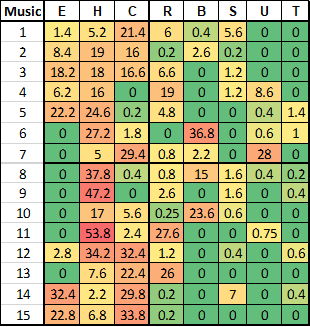
\includegraphics[width=4.5cm,height=4cm]{figures/Affects.png}
    \caption{The affect count averages per music file. Legend: (E)xcited, (H)appy, (C)ontented, (R)elaxed, (B)ored, (S)ad, (U)pset, (T)ense}
    \label{fig:affects}
    \end{minipage}
\end{marginfigure}

\begin{marginfigure}[-10pc]
\begin{minipage}{\marginparwidth}
     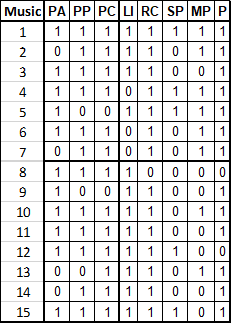
\includegraphics[width=4.75cm,height=7cm]{figures/Visualizations.png}
    \caption{The visualization attributes of each music file.}
    \label{fig:visualizations}
    \end{minipage}
\end{marginfigure}

\begin{marginfigure}[0pc]
\begin{minipage}{\marginparwidth}
     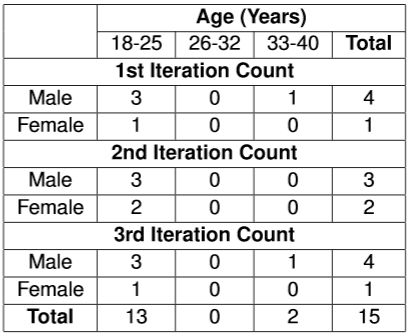
\includegraphics[width=4.5cm,height=4cm]{figures/demographic.png}
    \caption{The demographics of the participants in the experiments we conducted.}
    \label{fig:demographic}
    \end{minipage}
\end{marginfigure}



\subsection{Experiment Results and Findings}
A correlation analysis using Spearman's rho ($\rho$) was performed between the \textbf{affect data} (what the participants felt during certain points in the music) and \textbf{visualization attributes} (the characteristics of the visualizations), annotated with a music expert). The goal is to see if the affects felt by the testers coincide with certain visualization attributes. For each tester per music file, for each of the eight possible affects the tester was able to choose from, we counted how many times a button click corresponded to the feeling of such affect. We then took the average of each of the counts per affect per music file across all testers. Figure \ref{fig:affects} shows these affect count averages per music file.%  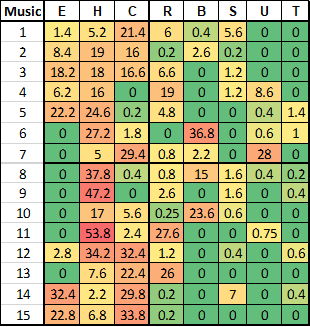
\includegraphics[width=4cm,height=4cm]{figures/Affects.png}
With the help of a music expert along with the qualitative descriptions of the DHH testers on the visualizations, we have identified key subjective visualization attributes. These attributes, along with their labels and ordinal values assigned, are:
\begin{enumerate}
    \item Particle activity (PA) - denotes whether the volume of particles emitted is sparse (0) or dense (1)
    \item Particle periodicity (PP) - denotes whether the particles are emitted irregularly (0) or regularly (1)
    \item Percussive coincidence (PC) - denotes whether the particles emit when and only when percussion is heard in the music (1) or not (0)
    \item Layer independence (LI) - denotes whether each visualization layer appears to be stacked (0) or independent of each other (1)
    \item Rectangle contiguity (RC) - denotes whether the appearance of contiguous groups of rectangles appear infrequently (0) or frequently (1)
    \item Star prominence (SP) - denotes whether the star visualizations are obscure (0) or prominent (1)
    \item Movement predictability (MP) - denotes whether the movement of the visualization is unpredictable (0) or predictable (i.e., when a pattern may be deduced) (1)
    \item Pulsation (P) - denotes whether the visualization layers appear to be rigid (0) or pulsating (1)
\end{enumerate}
Figures \ref{fig:prot3_1}, \ref{fig:prot3_2}, \ref{fig:prot3_3}, \ref{fig:lowparticle}, \ref{fig:lowstar}, and \ref{fig:highindependence} show examples of scenarios where certain visualization attributes were seen. In the first three figures, their implications on affect as observed in the analysis (described in the Experiment Results and Findings section) are also shown.

Figure \ref{fig:visualizations} shows the visualization attributes of each music file.

The Spearman's rank correlation coefficient is then calculated between the affect data and the visualization attributes. 

\begin{marginfigure}[-5pc]
\begin{minipage}{\marginparwidth}
     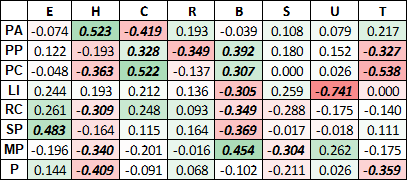
\includegraphics[width=4.75cm,height=2.3cm]{figures/AffectVisualization.png}
    \caption{The correlation values between the affect data and the visualization attributes.}
    \label{fig:correlation}
    \end{minipage}
\end{marginfigure}

\begin{marginfigure}[0pc]
\begin{minipage}{\marginparwidth}
     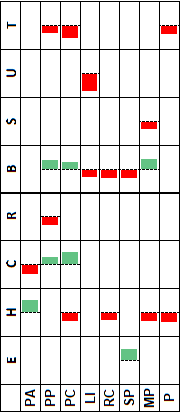
\includegraphics[width=4.5cm,height=8cm]{figures/TrendsNew_Rotated.png}
    \caption{The trends noted in the correlation between affect data and the visualization attributes. Green bars represent a direct relationship between a visualization attribute and an affect, while red bars represent inverse relationships between the same. The length of each bar denotes the strength of the correlation with the direction of the bar corresponding to whether it represents a direct relationship (to the right) or an inverse relationship (to the left). Note than only correlations with $|\rho| \geq 0.3$ (as per \cite{Cohen:1988}) are displayed.}
    \label{fig:trends}
    \end{minipage}
\end{marginfigure}

Figure \ref{fig:correlation} shows these correlation values wherein moderate and strong correlations (according to the standard of \cite{Cohen:1988}) are emphasized in order to highlight relationships wherein it may be hypothesized that the affects of the viewer are augmented by the visualizations. We have noted several trends from these correlations, as shown in Figure \ref{fig:trends}. For the affects observed to have at least moderately strong direct relationships with certain visualization attributes, it may be hypothesized that such visualization attributes \textit{induce} such affects. Likewise, for at least moderately strong inverse relationships observed, the pertinent visualization attributes are hypothesized to \textit{dissuade} the relevant affects. More comprehensive experiments and analyses are needed to confirm these relationships as well as to identify the specific moments in the music wherein such induction or dissuasion occurs.

% \begin{figure}[h]
%     \centering
%     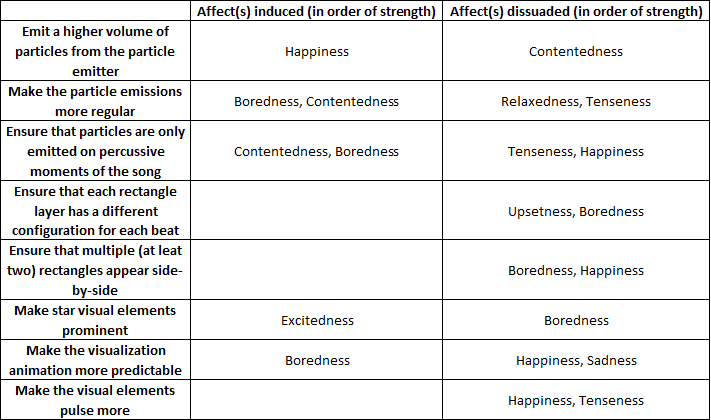
\includegraphics[width=9cm,height=6cm]{figures/Trends.png}
%     \caption{The trends noted in the correlation between affect data and the visualization attributes.}
%     \label{fig:trends}
% \end{figure}

\section{Conclusion and Future Work}
We have developed ViTune, a music visualization prototype for augmenting the musical experiences of the DHH, in collaboration with the DHH community. Our experiments suggest that for certain affects, the visualizations produced by the prototype at least moderately induce or dissuade such affects to the DHH. Our next step will be to determine exactly when and where in the music (and its visualizations) certain visual elements induce or dissuade such affects. This could be done by avoiding some of the subjective nature of determining relevant visual attributes through maintaining an internal visualization monitor which logs the visual elements currently shown along with their relevant objective measurements. This allows for viewing a \textit{snapshot} of the exact state of the visualizations the moment an affect is experienced, making it easier to infer the cause of the affect. Effectiveness studies between existing music visualizers and ViTune may be conducted to see how our tool fares against other visualizers and what functionalities ViTune could be incorporated from them with the guidance of the DHH community. Further work could also be done in integrating haptic devices to the system as well as integrating them into a user-ready music player software.

% \begin{marginfigure}[1pc]
% \begin{minipage}{\marginparwidth}
%      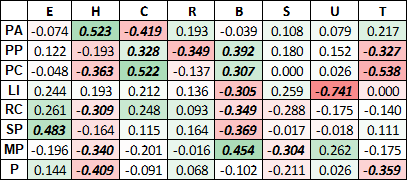
\includegraphics[width=4.75cm,height=2.25cm]{figures/AffectVisualization.png}
%     \caption{The correlation values between the affect data and the visualization attributes.}
%     \label{fig:correlation}
%     \end{minipage}
% \end{marginfigure}




% The next step will involve improving the visualization prototype based on insights acquired from the respondents throughout the first three (3) iterations of testing performed, as well as to package the prototype into a user-ready and functional web-based music visualization application.

% We plan to add further functionality to the current prototype based on the input gathered from past iterations of testing. An option to toggle the presence of accompanying haptic feedback is being considered for further development. Should additional visualization styles be developed, adding functionality to switch between multiple visualization styles is a possible addition to future iterations. As the lyrics feature in the current iteration is hardcoded due to time constraints in development, automated ways to extract lyrics (as applicable) from audio input are also being explored. 

% For additional iterations to be done in the future, we intend to conduct the testing with a larger number of participants. In order to accommodate the increased participant count, we are also considering more spacious venues for the experiments; where the visualizations may instead be projected in front of the participants rather than be presented through one machine for each participant. Testing will follow a modified protocol, which will primarily be based on what was used in the third iteration, and will take into account any constraints for testing new features which may be added to the application.


% \section{Future Impact}
% The impact we are hoping for in this research is to understand how visualizations, when used in order to enhance existing relevant interactions, are able to improve upon how the DHH are able to experience music through non-auditory means. We aim to integrate the visual aspect of music as an important element at par with lyrics, harmony, rhythm, and others in order to provide users with a richer understanding of musical works. We wish that this tool shall be used to lessen the alienation of music, and auditory-based works, in general towards the DHH community by providing them with a more visual representation of the said works. This visualization tool can be applied to further augment the musical experience of the hearing as a complement to the auditory means of experiencing music. Finally, the researchers are hoping that the concepts used in this study can be adapted and deployed by musical tools used by the musical community, not necessarily as a direct alternative, but as an accompaniment to their existing sets of features.

\section{Authors}
Jordan Aiko Deja is a faculty in the Software Technology Department, College of Computer Studies of De La Salle University, Manila, Philippines. He is also a PhD student at the University of Primorska, Koper, Slovenia. 

Jose Florencio Ciriaco IV, Alexczar Dela Torre, Carlo Miguel Eroles and Hans Joshua Lee are graduates of De La Salle University, with a Bachelor's Degree in Computer Science with specialization in Software Technology at De La Salle University Manila, Philippines.




\bibliographystyle{SIGCHI-Reference-Format}
\bibliography{sample}




\end{document}
    
% --------------------- v --- Template stuff --- v ----------------------------

% \section{Introduction}

% \section{ACM Copyrights \& Permission Policy}

% \section{Page Size}


% \section{Text Formatting}
% Please use an 8.5-point Verdana font, or other sans serifs font as
% close as possible in appearance to Verdana in which these guidelines
% have been set. Arial 9-point font is a reasonable substitute for
% Verdana as it has a similar x-height. Please use serif or
% non-proportional fonts only for special purposes, such as
% distinguishing \texttt{source code} text.

% \subsubsection{Text styles}
% The \LaTeX\ template facilitates text formatting for normal (for body
% text); heading 1, heading 2, heading 3; bullet list; numbered list;
% caption; annotation (for notes in the narrow left margin); and
% references (for bibliographic entries). Additionally, here is an
% example of footnoted\footnote{Use footnotes sparingly, if at all.}
% text. As stated in the footnote, footnotes should rarely be used.

% \begin{figure}
%   
\includegraphics[width=0.9\columnwidth]{figures/sigchi-logo}
%   \caption{Insert a caption below each figure.}~\label{fig:sample}
% \end{figure}

% \subsection{Language, style, and content}
% The written and spoken language of SIGCHI is English. Spelling and
% punctuation may use any dialect of English (e.g., British, Canadian,
% US, etc.) provided this is done consistently. Hyphenation is
% optional. To ensure suitability for an international audience, please
% pay attention to the following:

% \begin{table}
%   \centering
%   \begin{tabular}{l r r r}
%     % \toprule
%     & & \multicolumn{2}{c}{\small{\textbf{Test Conditions}}} \\
%     \cmidrule(r){3-4}
%     {\small\textit{Name}}
%     & {\small \textit{First}}
%       & {\small \textit{Second}}
%     & {\small \textit{Final}} \\
%     \midrule
%     Marsden & 223.0 & 44 & 432,321 \\
%     Nass & 22.2 & 16 & 234,333 \\
%     Borriello & 22.9 & 11 & 93,123 \\
%     Karat & 34.9 & 2200 & 103,322 \\
%     % \bottomrule
%   \end{tabular}
%   \caption{Table captions should be placed below the table. We
%     recommend table lines be 1 point, 25\% black. Minimize use of
%     table grid lines.}~\label{tab:table1}
% \end{table}

% \begin{itemize}\compresslist%
% \item Write in a straightforward style. Use simple sentence
%   structure. Try to avoid long sentences and complex sentence
%   structures. Use semicolons carefully.
% \item Use common and basic vocabulary (e.g., use the word ``unusual''
%   rather than the word ``arcane'').
% \item Briefly define or explain all technical terms. The terminology
%   common to your practice/discipline may be different in other design
%   practices/disciplines.
% \item Spell out all acronyms the first time they are used in your
%   text. For example, ``World Wide Web (WWW)''.
% \item Explain local references (e.g., not everyone knows all city
%   names in a particular country).
% \item Explain ``insider'' comments. Ensure that your whole audience
%   understands any reference whose meaning you do not describe (e.g.,
%   do not assume that everyone has used a Macintosh or a particular
%   application).
% \item Explain colloquial language and puns. Understanding phrases like
%   ``red herring'' requires a cultural knowledge of English. Humor and
%   irony are difficult to translate.
% \item Use unambiguous forms for culturally localized concepts, such as
%   times, dates, currencies, and numbers (e.g., ``1-5- 97'' or
%   ``5/1/97'' may mean 5 January or 1 May, and ``seven o'clock'' may
%   mean 7:00 am or 19:00). For currencies, indicate equivalences:
%   ``Participants were paid {\fontfamily{txr}\selectfont \textwon}
%   25,000, or roughly US \$22.''
% \item Be careful with the use of gender-specific pronouns (he, she)
%   and other gender-specific words (chairman, manpower,
%   man-months). Use inclusive language (e.g., she or he, they, chair,
%   staff, staff-hours, person-years) that is gender-neutral. If
%   necessary, you may be able to use ``he'' and ``she'' in alternating
%   sentences, so that the two genders occur equally
%   often~\cite{Schwartz:1995:GBF}.
% \item If possible, use the full (extended) alphabetic character set
%   for names of persons, institutions, and places (e.g.,
%   Gr{\o}nb{\ae}k, Lafreni\'ere, S\'anchez, Nguy{\~{\^{e}}}n,
%   Universit{\"a}t, Wei{\ss}enbach, Z{\"u}llighoven, \r{A}rhus, etc.).
%   These characters are already included in most versions and variants
%   of Times, Helvetica, and Arial fonts.
% \end{itemize}

% % \begin{figure}
% %   \includegraphics[width=.9\columnwidth]{figures/ea-figure2}
% %   \caption{If your figure has a light background, you can set its
% %     outline to light gray, like this, to make a box around
% %     it.}\label{fig:bats}
% % \end{figure}

% \begin{marginfigure}[-35pc]
%   \begin{minipage}{\marginparwidth}
%     \centering
%     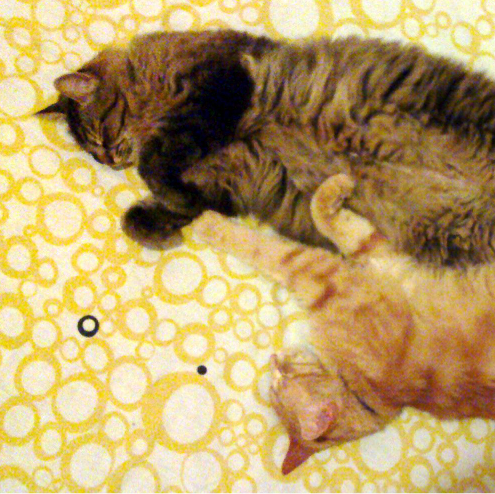
\includegraphics[width=0.9\marginparwidth]{figures/cats}
%     \caption{In this image, the cats are tessellated within a square
%       frame. Images should also have captions and be within the
%       boundaries of the sidebar on page~\pageref{sec:sidebar}. Photo:
%       \cczero~jofish on Flickr.}~\label{fig:marginfig}
%   \end{minipage}
% \end{marginfigure}

% \section{Figures}
% The examples on this and following pages should help you get a feel
% for how screen-shots and other figures should be placed in the
% template. Your document may use color figures (see
% Figures~\ref{fig:sample}), which are included in the page limit; the
% figures must be usable when printed in black and white. You can use
% the \texttt{\marginpar} command to insert figures in the (left) margin
% of the document (see Figure~\ref{fig:marginfig}). Finally, be sure to
% make images large enough so the important details are legible and
% clear (see Figure~\ref{fig:cats}).
% All figures should include alt text (figure description) for improved accessibility – see the Accessibility section.

% \section{Tables}
% You man use tables inline with the text (see Table~\ref{tab:table1})
% or within the margin as shown in Table~\ref{tab:table2}. Try to
% minimize the use of lines (especially vertical lines). \LaTeX\ will
% set the table font and captions sizes correctly; the latter must
% remain unchanged.

% \section{Accessibility}
% The Executive Council of SIGCHI has committed to making SIGCHI
% conferences more inclusive for researchers, practitioners, and
% educators with disabilities. As a part of this goal, the all authors
% are expected to work on improving the accessibility of their
% submissions. Specifically, we encourage authors to carry out the
% following five steps:
% \begin{itemize}\compresslist%
% \item Add alternative text (figure description) to all figures
% \item Mark table headings
% \item Generate a tagged PDF
% \item Verify the default language
% \item Set the tab order to ``Use Document Structure''
% \end{itemize}

% For links to detailed instructions and resources, please see:
% \url{http://chi2020.acm.org/authors/papers/guide-to-an-accessible-submission/}

% Unfortunately good tools do not yet exist to create tagged PDF files
% from Latex. \LaTeX\ users will need to carry out all of the above
% steps in the PDF directly using Adobe Acrobat, after the PDF has been
% generated.


% \begin{figure*}
%   \centering
%   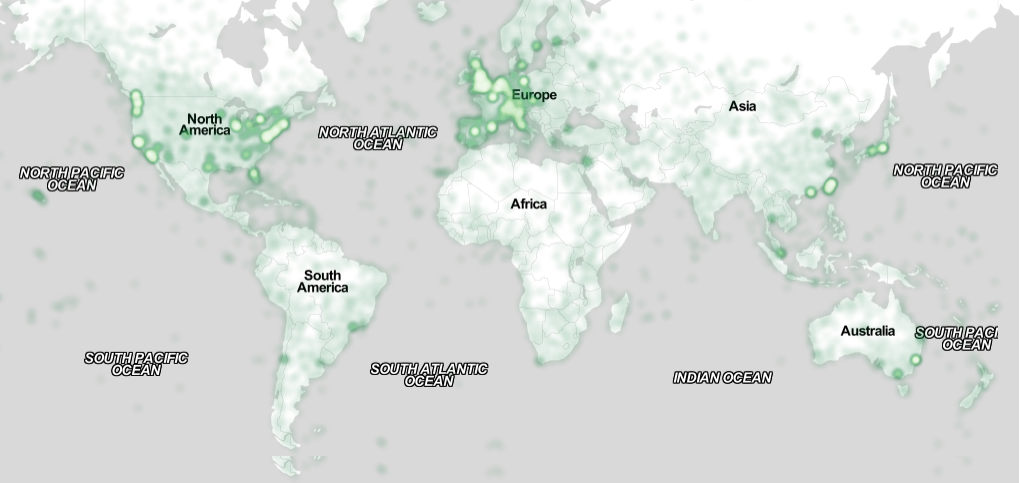
\includegraphics[width=1.3\columnwidth]{figures/map}
%   \caption{In this image, the map maximizes use of space. You can make
%     figures as wide as you need, up to a maximum of the full width of
%     both columns. Note that \LaTeX\ tends to render large figures on a
%     dedicated page. Image: \ccbynd~ayman on Flickr.}~\label{fig:cats}
% \end{figure*}

% \section{Producing and Testing PDF Files}
% We recommend that you produce a PDF version of your submission well
% before the final deadline. Your PDF file must be ACM DL Compliant and
% meet stated requirements,
% \url{http://www.sheridanprinting.com/sigchi/ACM-SIG-distilling-settings.htm}.

% \marginpar{\vspace{-23pc}So long as you don't type outside the right
%   margin or bleed into the gutter, it's okay to put annotations over
%   here on the left, too; this annotation is near Hawaii. You'll have
%   to manually align the margin paragraphs to your \LaTeX\ floats using
%   the \texttt{{\textbackslash}vspace{}} command.}

% \begin{margintable}[1pc]
%   \begin{minipage}{\marginparwidth}
%     \centering
%     \begin{tabular}{r r l}
%       & {\small \textbf{First}}
%       & {\small \textbf{Location}} \\
%       \toprule
%       Child & 22.5 & Melbourne \\
%       Adult & 22.0 & Bogot\'a \\
%       \midrule
%       Gene & 22.0 & Palo Alto \\
%       John & 34.5 & Minneapolis \\
%       \bottomrule
%     \end{tabular}
%     \caption{A simple narrow table in the left margin
%       space.}~\label{tab:table2}
%   \end{minipage}
% \end{margintable}
% Test your PDF file by viewing or printing it with the same software we
% will use when we receive it, Adobe Acrobat Reader Version 10. This is
% widely available at no cost. Note that most
% reviewers will use a North American/European version of Acrobat
% reader, so please check your PDF accordingly.

% \section{Acknowledgements}
% We thank all the volunteers, publications support, staff, and authors
% who wrote and provided helpful comments on previous versions of this
% document. As well authors 1, 2, and 3 gratefully acknowledge the grant
% from NSF (\#1234--2222--ABC). Author 4 for example may want to
% acknowledge a supervisor/manager from their original employer. This
% whole paragraph is just for example. Some of the references cited in
% this paper are included for illustrative purposes only.

% \section{References Format}
% Your references should be published materials accessible to the
% public. Internal technical reports may be cited only if they are
% easily accessible and may be obtained by any reader for a nominal
% fee. Proprietary information may not be cited. Private communications
% should be acknowledged in the main text, not referenced (e.g.,
% [Golovchinsky, personal communication]). References must be the same
% font size as other body text. References should be in alphabetical
% order by last name of first author. Use a numbered list of references
% at the end of the article, ordered alphabetically by last name of
% first author, and referenced by numbers in brackets. For papers from
% conference proceedings, include the title of the paper and the name of
% the conference. Do not include the location of the conference or the
% exact date; do include the page numbers if available. 

% References should be in ACM citation format:
% \url{http://www.acm.org/publications/submissions/latex_style}.  This
% includes citations to Internet
% resources~\cite{CHINOSAUR:venue,cavender:writing,psy:gangnam}
% according to ACM format, although it is often appropriate to include
% URLs directly in the text, as above. Example reference formatting for
% individual journal articles~\cite{ethics}, articles in conference
% proceedings~\cite{Klemmer:2002:WSC:503376.503378},
% books~\cite{Schwartz:1995:GBF}, theses~\cite{sutherland:sketchpad},
% book chapters~\cite{winner:politics}, an entire journal
% issue~\cite{kaye:puc},
% websites~\cite{acm_categories,cavender:writing},
% tweets~\cite{CHINOSAUR:venue}, patents~\cite{heilig:sensorama}, 
% games~\cite{supermetroid:snes}, and
% online videos~\cite{psy:gangnam} is given here.  See the examples of
% citations at the end of this document and in the accompanying
% \texttt{BibTeX} document. This formatting is a edited version of the
% format automatically generated by the ACM Digital Library
% (\url{http://dl.acm.org}) as ``ACM Ref''. DOI and/or URL links are
% optional but encouraged as are full first names. Note that the
% Hyperlink style used throughout this document uses blue links;
% however, URLs in the references section may optionally appear in
% black.

\balance{} 

\bibliographystyle{SIGCHI-Reference-Format}
\bibliography{sample}

\end{document}

%%% Local Variables:
%%% mode: latex
%%% TeX-master: t
%%% End:
